
\documentclass[11pt, oneside, dvipdfmx]{book}
\newcommand{\folder}{/home/bohulu/Documents/texmf}
%\newcommand{\folder}{/home/hanchenggao/Documents/texmf}
\input{\folder/hfiles/epaper}
%\renewcommand{\thesubsubsection}{\Alph{subsubsection}.}
%\setcounter{secnumdepth}{3}
%\usepackage[ruled,vlined]{algorithm2e}
\usepackage {graphics}
\usepackage{caption}
\usepackage{tabularx}
%\usepackage {graphics}
%\setCJKmainfont{SimSun}
\begin{document}
\title{
A Novel Method for Obtaining the Pattern of Low-Weight Codeword Components of Recursive Systematic Convolutional Codes}
\author{Kwame Ackah Bohulu}
\date{\today}
\maketitle
\newpage
%Knowledge of the distance spectrum, as well as the structure of the message inputs that make up the distance spectrum for a specific recursive systematic convolutional (RSC) code is vital to the design of Turbo Code interleavers. Even though the distance spectrum of an RSC code can be obtained by calculating its transfer function, it does not provide any information about the structure of the message inputs. %and the complexity involved in calculating the transfer function increases with the number of states of the RSC code.
%%%%%%%%%%%%%%%%%%%%%%%%%%%
\section{Abstract}
In this paper, we present a novel low-complexity method for obtaining the pattern of low-weight codeword components for a given recursive systematic convolutional code. %Our proposed method makes it easy to determine which RSC codes
We generate a low-weight codeword component pattern list for selected recursive systematic convolutional codes and validate our proposed method by obtaining a union bound, which we compare to simulation results and the union bound obtained via the transfer function method. From the results, we are able to determine which recursive systematic convolutional codes are best suited for use in turbo codes.
\newpage
\section{Introduction}

\begin{enumerate}
\item The {\it turbo code} (TC) \cite{ref1}, introduced by Claude Berrou 
\begin{itemize}
\item Excellent  \textit{forward-error correcting} (FEC) code

\item Applications include :LTE standard, IEEE 802.16 WiMAX (worldwide interoperability for microwave access) and DVB-RCS2 (2nd generation digital video broadcasting - return channel via satellite) standards \cite{ref7}.
\end{itemize}


 \item Construction of a TC 
 \begin{itemize}
 \item  Two {\it recursive systematic convolutional} (RSC) codes concatenated via an interleaver
 
 \item Good performance of TC due to interleaver. 
 \end{itemize}


\item Good deterministic interleaver design requirements?
\begin{itemize}
\item complete knowledge of all the low-weight codeword component patterns in the RSC code

\item missing even one of these patterns can create sub-par interleaver and TC

\end{itemize}

\item Interleaver Design Tools?
\begin{itemize}
\item The transfer function of an RSC code provides information about the distance spectrum.

\item No information with regards to the pattern of the low-weight codeword components.

\item Complexity increases with the number of states of RSC code.

\item No interleaver design tool reveals distance spectrum and the low-weight codeword component patterns.

\item As a result, many interleaver design methods completely ignoring certain important low-weight codewords, example \cite{ref5}. 
\end{itemize}


\item Acheivements of this research
\begin{itemize}
\item We propose a novel method for revealing the pattern of the low-weight codeword components. 

\item  Excellent interleaver design tool

\item Complexity independent of RSC code states
\end{itemize}
\end{enumerate}
%We generate a low-weight codeword component pattern list for specific RSC codes and obtain union bounds using our proposed method. We then validate our method by comparing the proposed union bounds to simulation results and the union bounds obtained via the transfer function method.

%The remainder of the research paper is organised as follows. Definitions used in the research paper are introduced in Section \ref{secPrelim}. In Section \ref{sec2}, we establish the theoretical foundations for our novel method by discussing the characteristics of the low-weight codewords. Then in Section \ref{sec3}, we present our novel method and use examples to clarify the workings of our proposed method. Validation of our proposed method for specific RSC codes as well as discussion related to turbo code interleaver design is done in Section \ref{sec4} and the paper concludes in Section \ref{sec6}.

\subsection{Notations}
\begin{enumerate}
\item  least common multiple of integers $\alpha$ and $\beta$ : $\lcm(\alpha,\beta)$
\item remainder $\alpha$ divided by $\beta,~\beta \neq 0$ : $\alpha \mod \beta$
\item $\alpha$ is a divisor of $\beta$: $\alpha | \beta$ 
\item shorthand for the operation $(\alpha \bmod \epsilon_0,~\beta \bmod \epsilon_0)$ : $(\alpha,~\beta) \bmod $, $(\alpha,~\beta)$ are integer pairs.
\item tensor product that yields the set consisting of all pairs of $\cM$ and $\cN$ : $\cM \otimes \cN$, $\cM$ and $\cN$ are integer sets.
\end{enumerate}



\newpage
\section{Preliminaries}
\label{secPrelim}

\begin{enumerate}
\item A polynomial in $x$ with degree $M$ is an expression of the form
\begin{equation}
v(x) = \sum_{m=0}^{M} v_mx^m
\label{Eq:polynomial}
\end{equation}
where $v_m,~0 \leq m \leq M$, are called the \textit{coefficients} and $v_M \neq 0$. If $v_M=1,~v(x)$ is called a \textit{monic} polynomial. 

\item We call the total number of the non-zero coefficients the \textit{Hamming weight} of $v(x)$, denoted as $w_H(v(x))$.

\item For a prime number $p$, if the addition and multiplication of two elements in the integer set $\{ 0,1,p-1\}$ are performed on the terms $\bmod~p$, we call the set a Galois field, denoted as $\GF(p)$. If the coefficients in \eqref{Eq:polynomial} are elements of $\GF(p)$, $v(x)$ is called a {\it polynomial over} $\GF(p)$.

\item For two polynomials $v(x)$ and $w(x)$ with degrees $M$ and $N$, respectively, the addition and multiplication over $\GF(p)$ are defined as 
\begin{align}
v(x)+w(x)=\sum_{m=0}^{\max\{ M,N\}} [(v_m +w_n)\mod p] x^m
\label{Eq:addition}
\end{align}
and
\begin{align}
v(x)w(x)=\sum_{m=0}^{ M+N} \sum_{i=0}^{m} [v_i w_{m-i}\mod p]x^m
\label{Eq:multiplication}
\end{align}
respectively. 

\item We say a monic polynomial is a \textit{prime polynomial} if it cannot be obtained by the multiplication of some lower degree polynomials.

\item For two polynomials $v(x)$ and $w(x)$ over $\GF(p)$, $w(x) \neq 0$, there exists polynomials $q(x)$ and $r(x)$ 
over $\GF(p)$ such that 
\begin{align}
v(x) = w(x)q(x)+r(x)
\label{Eq:decomposition}
\end{align}
with $\deg(r(x)) < \deg(w(x))$. We represent $r(x)$ in the expression \eqref{Eq:decomposition} as
\begin{align}
r(x) \equiv v(x)\mod w(x)
\end{align}
and call it the \textit{remainder polynomial}, while $q(x)$ is called the \textit{quotient polynomial} of the division of $v(x)$ by $w(x)$.

\item Let $v(x)$ be a prime polynomial over $\GF(p)$ with $\deg(v(x)):=M>1$ and $\cV$ be the set of size $p^M$ containing all polynomials over $\GF(p)$ with degree less than $M$. Then, the \textit{extension field of $\GF(p)$}, denoted by $\GF\left(p^M\right)$, is the set $\cV$ with addition and multiplication over $\GF(p)$, where the multiplication is carried out modulo-$v(x)$ over $\GF(p)$.

\item Each non-zero element in $\GF \left(p^M\right)$ can be represented by a power of $x$ uniquely as $x^m,~0 \leq m \leq p^M-1$. 

\item For each non-zero element of $\GF \left(p^M\right)$, there exist integers $\epsilon$ such that $x^{\epsilon}=1$ and the least positive integer among them is called the \textit{order} of $x$. We say that elements with order $\epsilon=p^M-1$ are \textit{primitive elements}. 

\item For $\GF \left(p^M\right)$ generated by a prime polynomial $v(x)$ with $\deg(v(x))=M$, if $x$ is a primitive element in $\GF \left(p^M\right)$, then  $v(x)$ is called a \textit{primitive polynomial}. 
%

\item Finally, the root of $v(x)$, is the non-zero element $\varphi,~\varphi \in \GF \left(p^M\right)$ such that $v(\varphi)=0$. If $v(x)$ is a primitive polynomial, the order of $\varphi$ is $\epsilon=p^M-1$, otherwise $\epsilon | p^M-1$. 
Moreover, the elements $\varphi^i,~0 \leq i \leq \epsilon -1$, are all distinct from each other.
 \end{enumerate}
%Finally, let $(e,~f)$ represent a pair of non-zero positive integers. Then $(e,~f) \bmod 2^M-1$ is shorthand for the operation $(e \bmod 2^M-1,~f \bmod 2^M-1)$.


\newpage
\section{The characteristics of the low-weights codewords of RSC code}
\label{sec2}
\begin{enumerate}
\item The outputs of an RSC code are determined by the input bit sequence $b(x)$, the states of the shift registers and the feedforward and feedback connections of the shift registers that can be represented by a generator function. 

\item As an instance,  the generator function of a rate $1/2$ RSC code may be written as  $$\left[1 ~\frac{f(x)}{g(x)}\right]$$ where $1$ yields the \textit{systematic  component} (SC) $b(x)$ while the \textit{parity-check component} (PC) $h(x)$ is associated with the feedforward and feedback connections of the shift registers, specified by $f(x)$ and $g(x)$, respectively. 

\item The outputs $c(x)$ are the mixture of the SC and PC as
\begin{equation}
c(x) = b(x^2)+xh(x^2)
\label{codeword-comp}
\end{equation}
where 
\begin{equation}
h(x) =f(x)g^{-1}(x)b(x)
\label{eq:parity-def}
\end{equation}
From \eqref{codeword-comp}, it is trivial that
\begin{equation}
w_H(c(x))=w_H(b(x)) + w_H(h(x))
\label{eq:cw-weight}
\end{equation}
and hence, each low-weight codeword is combination of low-weight SC and PC.

\item Under the assumption of large frame sizes, the presence of $g^{-1}(x)$  in \eqref{eq:parity-def} may involve a particular bit sequence that repeats a large number of times, hence yielding a high-weight PC. 

\item Low-weight PCs occur if and only if
\begin{equation}
b(x) \bmod g(x) \equiv 0
\label{eq:rtz-input}
\end{equation}

\item The SCs satisfying \eqref{eq:rtz-input} are called \textit{return-to-zero} (RTZ) inputs. Thus, every RTZ input can be factorized as  
\begin{equation}
b(x) =a(x)g(x)
\label{eq:low-weight-msg}
\end{equation}
and, substituting (\ref{eq:low-weight-msg}) into \eqref{eq:parity-def}, we can characterize the low-weight PC as
\begin{equation}
\begin{split}
h(x)&=f(x)\cdot g^{-1}(x)\cdot a(x)g(x)\\
&=a(x)f(x)
\end{split}
\label{eq:low-weight-parity}
\end{equation}

\item Therefore, in this paper, we attempt to find $a(x)$s satisfying  \eqref{eq:low-weight-msg} and  \eqref{eq:low-weight-parity} simultaneously for low-weight $b(x)$ and $h(x)$, respectively. 
%
However, since there is no essential mathematical difference between the two equations, in the next section, we present a method for determining the low-weight PC patterns for $2 \leq w_H(h(x)) \leq 3$.
\end{enumerate}



\newpage
%\section{Novel Method to Determine the Low-Weight Parity-Check Pattern}
\label{sec3}
In this section, we present our novel method for obtaining what we have named the \textit{codeword pattern distance spectrum}. Compared to the transfer function method, its complexity is independent of the number of states of the RSC. It is also able to reveal the pattern of low-weight codewords. Our novel method can be seen as the combination of two different but related methods. The first method is quite simple and makes use of the fact that in the polynomial domain, RTZ inputs and their corresponding parity-check sequences share a common factor. 
The second method shows how to obtain this common factor when the weight of the parity-check sequence is fixed for a given RSC code. 
%After explaining the inner working of our novel method, we used it to obtain the partial codeword pattern distance spectrum for the $5/7,~ 37/21$ and $23/35$  RSC codes.



\subsection{Low-weight Codewords}
%(quarantine)%The distance spectrum derived via the transfer function method is an insufficient tool when it comes to to interleaver design. In this section, we present a novel method that generates what we refered to as the structured distance spectrum, which is the distance spectrum with the structure of the RTZ inputs as well as the corresponding parity-check sequence revealed, therefore making it a very useful tool for interleaver design.

%(quarantine)%For an RSC code, the Hamming weight of the codeword $w_H(\bc)$ is the sum of the weights of the parity bit sequence and message input. 
The parity-check sequence can be expressed as 
\begin{equation}
h(x) =f(x)\cdot g^{-1}(x)\cdot b(x)
\label{novelEq0}
\end{equation}
If we consider large frame sizes, the presence of $g^{-1}(x)$ means that within $h(x)$ is a particular sequence of bits that is repeated a large number of times. This results in a large parity weight, and by extension, a relatively high-weight codeword. The only time this is not the case is when
\begin{equation}
b(x) \bmod g(x) \equiv 0
\label{novelEq1}
\end{equation}
This results in a relatively low-weight parity bit sequence, which might produce a low-weight codeword. Any $b(x)$ that meets the condition in (\ref{novelEq1}) can be written as 
\begin{equation}
b(x) =a(x)g(x)
\label{novelEq2}
\end{equation}
where $a(x)$ is a monic polynomial with the coefficient of the lowest term not equal to $0$.
By fixing $b(x)$ from (\ref{novelEq2}) into (\ref{novelEq0}), we have 
\begin{equation}
\begin{split}
h(x)&=f(x)\cdot g^{-1}(x)\cdot a(x)g(x)\\
&=a(x)f(x)
\end{split}
\label{novelEq3}
\end{equation}
%(quarantine)%Using both (\ref{novelEq2})  and (\ref{novelEq3}), we wish to list all low-weight codewords for a given RSC code.A low-weight codeword is any codeword which satisfies the condition, $w_H(\bc) \leq d_{\text{max}}$. This list is known as the \textit{partial structured distance spectrum}. To generate the partial structured distance spectrum, we take note of a few things. 

%From (\ref{novelEq2})  and (\ref{novelEq3}), we observe that $a(x)$ is a common factor in both equations and if we are able to solve for $a(x)$ via either of the equations, the remaining equation can be solved. To solve for $a(x)$ requires that in either equation, it should be the only unknown variable. At first glance, it might seem that $g(x)$ and $f(x)$ are the only known variables because they are dependent on the RSC code in question. However, if we remember that the weight of $h(x)$ and $b(x)$ is directly proportional to the number of terms it has, then we are on our way to obtain our second known variable. What is left is to determine the valid power values for the polynomial  terms, depending on the weight of $h(x)$ or $b(x)$.

Revisiting (\ref{novelEq3}), once $f(x)$ is given, our goal is to find $a(x)$ that results in a low-weight $h(x)$. To this end, we consider the roots of $f(x)$ 
%If $f(x)$ is a prime polynomial or can be factorized into prime polynomials, the the roots of $f(x)$ are its primitive elem
 %denoted by $\beta_i,~ 0 \leq i < 2^{m}-1)$. Then it is obvious that $h(\beta^i)=0$~ for all $\beta^i$ that are primitive elements 
and we can reformulate our goal as to find weight-$w$ polynomials ($h(x)$) which take all the roots of $f(x)$ as its roots. The roots of $f(x)$ depend on its characteristic make-up and once that is known, we can easily determine the structure of $h(x)$ for a given value of $w_H(h(x))$. 
The characteristic make-up of $f(x)$ can be grouped into the three cases below. 
\begin{enumerate}
\item Single primitive polynomial.
\item Prime but not a primitive polynomial.
\item Made up of repeated polynomial roots.
\end{enumerate}
We present a method for determining valid values of $h(x)$ for a given RSC code when $2 \leq w_H(h(x))\leq 3$. It is worth noting that the method to be discussed can also be used to obtain valid values of $b(x)$, because there is no difference between the general structure of $h(x)$ and $b(x)$ once the Hamming weight is fixed. 
\subsection{The patterns of the weight-2 PCs}
\label{sec:PC2}
Each weight-2 PC can be written as 
\begin{equation}
h(x)=1+x^a
\label{eq:wt2-gen-form}
\end{equation}
without loss of generality. Thus, we have from \eqref{Eq:rootcondition} that
\begin{equation}
(\beta_0^i)^a =1,~~~ 0 \leq i < \epsilon_0
\label{novelEq5b}
\end{equation}
On the other hand, the order $\epsilon_0$ is the least integer satisfying $\beta_0^{\epsilon_0} \equiv 1$, thus, $a$ should satisfy the condition
$$a \bmod \epsilon_0  \equiv 0$$

\begin{example}$f(x)=1+x+x^2$.\newline 
For this case, since $x^1=x$, $x^2 \equiv 1+x$, and $x^3 \equiv 1 \bmod f(x)$, the order of the root $\beta_0$ is $\epsilon_0=3$ and $a$ should be a multiple of $3$. The corresponding values for $a(x)$ and $h(x)$ are shown in Table \ref{novelTab2} for the first four valid values of $a$.
\begin{table}[htbp]
%\parbox{.5\linewidth}{
 \caption{$f(x)=1+x+x^2$}
\centering
 \begin{tabular}{c c c} 
%\hline
 $a(x)$ & $h(x)$ \\ [0.5ex] 
 \hline\hline
$1+x$
 & $1+x^{3}$ \\
\hline
$1+x+x^3+x^4$
 & $1+x^{6}$ 
 \\
\hline
$1+x+x^3+x^4+x^6+x^{7}$ 
&  $1+x^{9}$ 
\\
\hline
$1+x+x^3+x^4+x^6+x^{7}+x^9+x^{10}$
 &  $1+x^{12}$ \\
 \end{tabular}
 \label{novelTab2}
\end{table}
\label{ex-2}

We may write the weight-2 PCs in general form as $h(x)=1+x^{3\ell},~\ell>1$ and the corresponding $a(x)$ is given by 
\begin{equation*}
a(x)=\sum_{\ell=0}^{L-1} x^{3\ell}(1+x)
\end{equation*}
\label{ex-1}
\end{example}




\begin{example}
$f(x)=1+x+x^2+x^3+x^4$\newline
We can confirm that the order of $\beta_0$ is $\epsilon_0=5$. This means that $a$ should be a multiple of $5$. The corresponding values for $a(x)$ and $h(x)$ are shown in Table \ref{novelTab3} with general forms for $\ell>1$

%}
\begin{table}[htbp]
%\parbox{.5\linewidth}{
\caption{$f(x)=1+x+x^2+x^3+x^4$}
\centering
\begin{tabular}{c c} 
 \hline
 $a(x)=\sum_{\ell=0}^{L-1} x^{5\ell}(1+x)$ & $h(x)=1+x^{5\ell}$  \\ [0.5ex] 
 \hline\hline
$1+x$ &$1+x^5$\\ 
$1+x+x^5+x^6$ &$1+x^{10}$  \\
$1+x+x^5+x^6+x^{10}+x^{11}$ & $1+x^{15}$ \\
$1+x+x^5+x^6+x^{10}+x^{11}+x^{15}+x^{16}$ &$1+x^{20}$  
 \end{tabular}
 \label{novelTab3}
%}ll
\end{table}
\label{ex-2}
\end{example}

\begin{example}
	$f(x)=1+x^2$\newline
	Since 
	\[
	f(x)=(1+x)^2\]
	and the order of the root $\beta_0=1$ is $\epsilon_0=1$, we obtain from \eqref{Eq:rootcondition} and \eqref{Eq:differential}
	\begin{align}
		(\beta_0)^a = 1
		\label{Eq:example31}
	\end{align}
	\begin{align}
		a(\beta_0)^{(a-1)} = 0
		\label{Eq:example32}
	\end{align}	
	Although \eqref{Eq:example31} indicates $a$ can be any positive integer, we can see from \eqref{Eq:example32} that $a$ should be even number.
	The corresponding values for $a(x)$ and $h(x)$ are shown in Table \ref{novelTab1} with general forms for $\ell>1$.
	\begin{table}[htbp]
		\renewcommand{\arraystretch}{1.3}
		%\parbox{.3\linewidth}{
		\caption{$f(x)=1+x^2$}
		\centering
		\begin{tabular}{c c } 
			\hline
			$a(x)=\sum_{\ell=0}^{L-1} x^{2\ell}$ & $h(x)=1+x^{2\ell}$ \\ [0.5ex] 
			\hline\hline
			$1$ & $1+x^2$\\ 
			$1+x^2$ & $1+x^4$ \\
			$1+x^2+x^4$ & $1+x^6$\\
			$1+x^2+x^4+x^6$ & $1+x^8$ 
		\end{tabular}
		\label{novelTab1}
	\end{table}
\label{ex-3}
\end{example}



---------------------------
%=====================Deleted Examples  =======================%
%\begin{example}
%$f(x)=1+x^2+x^3+x^4$\newline
%$f(x)$ can be written as 
%$$f(x)=\prod_{k=0}^{1}f_k(x)$$
%where 
%$$f_0(x)=1+x,~f_1(x)=1+x+x^3$$ 
%For $f_0(x), x \equiv 1$, and $x^1 \equiv 1 \bmod f_0(x)$, which means the order of the root $\beta_0$ is $\epsilon_0=1$ and $a_0$ should be a multiple of $1$. Again, for  $f_1(x), x^3 \equiv 1+x$, and $x^7 \equiv 1 \bmod f_1(x)$, which means the order of the root $\beta_1$ is $\epsilon_1=7$ and $a_1$ should be a multiple of $7$.
%Finally, valid values of $a$ should be a multiple of the least common multiples of $a_0$ and $a_1$, which means $a$ should be a multiple of $7$.
%The corresponding values for $a(x)$ and $h(x)$ are shown in Table \ref{novelTab1-a} with general forms for $\ell>1$.
%\begin{table}[htbp]
%\renewcommand{\arraystretch}{1.3}
%\parbox{.3\linewidth}{
 %\caption{$f(x)=1+x^2+x^3+x^4$}
 %\centering
%\begin{tabular}{c c } 
%\hline
 %$a(x)=\sum_{\ell=0}^{L-1} x^{7\ell}(1+x^2+x^3)$ & $h(x)=1+x^{7\ell}$ \\ [0.5ex] 
%\hline\hline
%$1+x^2+x^3$ & $1+x^7$\\ 
%$1+x^2+x^3+x^7+x^9+x^{10}$ & $1+x^{14}$ \\
%$1+x^2+x^3+x^7+x^9+x^{10}+x^{14}+x^{16}+x^{17}$ & $1+x^{21}$
%\end{tabular}
% \label{novelTab1-a}
%\end{table}
%\end{example}

%\begin{example}
%$f(x)=1+x+x^2+x^3+x^4+x^5+x^6$\newline
%$f(x)$ can be written as 
%$$f(x)=\prod_{k=0}^{1}f_k(x)$$
%where 
%$$f_0(x)=1+x^2+x^3,~f_1(x)=1+x+x^3$$ 
%For $f_0(x), x^3 \equiv x^2+1$, and $x^7 \equiv 1 \bmod f_0(x)$, which means the order of the root $\beta_0$ is $\epsilon_0=7$ and $a_0$ should be a multiple of $7$. Again, for  $f_1(x), x^3 \equiv 1+x$, and $x^7 \equiv 1 \bmod f_1(x)$, which means the order of the root $\beta_1$ is $\epsilon_1=7$ and $a_1$ should be a multiple of $7$.
%Finally, valid values of $a$ should be a multiple of the least common multiples of $a_0$ and $a_1$, which means $a$ should be a multiple of $7$.
%The corresponding values for $a(x)$ and $h(x)$ are shown in Table \ref{novelTab1-b} with general forms for $\ell>1$.
%\begin{table}[htbp]
%\renewcommand{\arraystretch}{1.3}
%\parbox{.3\linewidth}{
% \caption{$f(x)=1+x+x^2+x^3+x^4+x^5+x^6$}
 %\centering
%\begin{tabular}{c c } 
%\hline
 %$a(x)=\sum_{\ell=0}^{L-1} x^{7\ell}(1+x)$ & $h(x)=1+x^{7\ell}$ \\ [0.5ex] 
%\hline\hline
%$1+x$ & $1+x^7$\\ 
%$1+x+x^7+x^8$ & $1+x^{14}$ \\
%$1+x+x^7+x^8+x^{14}+x^{15}$ & $1+x^{21}$
%\end{tabular}
% \label{novelTab1-b}
%\end{table}
%\end{example}
%=====================================End of deleted examples========================%
\begin{example}
$f(x)=1+x^2+x^3+x^4+x^6$\newline
$f(x)$ can be written as 
$$f(x)=\prod_{k=0}^{1}f_k(x)$$
where 
$$f_0(x)=1+x+x^2,~f_1(x)=1+x+x^2+x^3+x^4$$ 
From Example \ref{ex-1} and Example \ref{ex-2}, we know that $a_0=3$ and $a_1=5$.
Hence, valid values of $a$ should be a multiple of the least common multiples of $a_0$ and $a_1$, which means $a$ should be a multiple of $15$.
The corresponding values for $a(x)$ and $h(x)$ are shown in Table \ref{novelTab1-c} with general forms for $\ell>1$.
\begin{table}[htbp]
\renewcommand{\arraystretch}{1.3}
%\parbox{.3\linewidth}{
 \caption{$f(x)=1+x^2+x^3+x^4+x^6$}
 \centering
\begin{tabular}{c c } 
\hline
 $a(x)=\sum_{\ell=0}^{L-1} x^{15\ell}(1+x^2+x^3+x^6+x^7+x^9)$ & $h(x)=1+x^{15\ell}$ \\ [0.5ex] 
\hline\hline
$1+x^2+x^3+x^6+x^7+x^9$ & $1+x^{15}$\\ 
$1+x^2+x^3+x^6+x^7+x^9+x^{15}+x^{17}+x^{18}+x^{21}+x^{22}+x^{24}$ & $1+x^{30}$ \\
\end{tabular}
 \label{novelTab1-c}
\end{table}

%We may write the weight-2 PCs in general form as $h(x)=1+x^{7\ell},~\ell>1$ and the corresponding $a(x)$ is given by 
%\begin{equation*}
%a(x)=\sum_{\ell=0}^{L-1} x^{7\ell}(1+x)
%\end{equation*}
\end{example}



\subsection{The patterns of the weight-3 PCs}
Each weight-3 PC can be written as 
\begin{equation}
h(x)=1+x^a+x^b,~a\neq b
\label{novelEqwt3}
\end{equation}
without loss of generality. 
Fixing $\beta_0$ into $h(x)$ we have
\begin{equation}
\beta_0^a+\beta_0^b= 1
\label{novelEq5b}
\end{equation}

To solve \eqref{novelEq5b}, we refer to the table of the extended field for GF$(2^M)$, and we can find the valid $(\eta,~\zeta)$ pairs $\st X^{\eta}+X^{\zeta}=1$. If there are no valid $(\eta,~\zeta)$ pairs, then there is no parity check component of weight $3$ for the given $f(x)$. Depending on the Galois field, there might be multiple values of $(\eta,~\zeta)$ that satisfy \eqref{novelEq5b},
 so we represent the set of all $(\eta,~\zeta)$ pairs by $\cZ$. Then, any valid value $(a,~b)$ values should satisfy the condition
\begin{equation}
(a,b) \equiv (\eta,~\zeta) \bmod \epsilon_0,~(\eta,~\zeta)\in \cZ
\end{equation}
% since $\beta^{2^{m}-1}=1$.
\begin{example}
$f(x)=1+x+x^2$ \newline
The elements of GF$(2^2)$ are shown in Table \ref{novelTab7} and it is obvious that $\cZ=\{(1,2)\}$.
This means that $(a,b) = (3\ell+1,~3n+2),~l=n=\left\{0,1,...\right\}$.  The corresponding values for $a(x)$ and $h(x)$ are shown in the table below for the first four valid values of $(a,b)$.
\label{ex-5}
\end{example}

 \begin{table}[htbp]
 \caption{Non-zero Elements of GF$(2^2)$ generated by $f(x)=1+x+x^2$}
\centering
 \begin{tabular}{c c} 
 \hline
 power representation & actual value \\ [0.5ex] 
 \hline\hline
$X^0~=X^3=1$ & $1$\\
\hline
$X$ & $x$\\
\hline
$X^2$ &  $1+x$\\
\hline
 \end{tabular}
 \label{novelTab7}
\end{table}

\begin{table}[htbp]
 \caption{$f(x)=1+x+x^2$}
\centering
 \begin{tabular}{c c} 
 \hline
 $a(x)$ & $h(x)$\\ [0.5ex] 
 \hline\hline
$1$ & $1+x+x^2$\\ 
\hline
$1+x+x^2$ &  $1+x^2+x^4$\\
\hline
$1+x+x^3$ & $1+x^4+x^5$\\
\hline
$1+x^2+x^3$ & $1+x+x^5$ 
 \end{tabular}
 \label{novelTab8}
\end{table}

We may write the weight-3 PCs in general form as $h(x)=1+x^{3\ell+1}+x^{3n+2},~\ell,~n \geq 0$ 
%and the corresponding $a(x)$ is given by 
%\begin{equation*}
%a(x)=\sum_{\ell=0}^{L-1} x^{3\ell}(1+x)
%\end{equation*}
%\label{ex-1}



\paragraph{Case2}$f(x)$ can be factorised into multiple irreducible polynomials. \newline
For this case, we can write $f(x)$ as $$f(x)=\prod_{k=1}^{K}f_k(x)$$ where $f_k(x)$ is an irreducible polynomial of order $M_k$ with root $\beta \in $ GF$(2^{M_k})$, $\beta^{\epsilon_k}=1$. 
For each $f_k(x)$, we refer to the table of the extended field it generates and form the set $\cZ_k$, which contains all the valid $(\eta^{(k)},~\zeta^{(k)})$ pairs for that particular $f_k(x)$. If that set exists, then, for that $f_k(x)$ the following condition is met
\begin{equation}
\cA\cB_k=\{(a_k,~b_k)~|~(a_k,~b_k) \equiv (\eta^{(k)},~\zeta^{(k)}) \bmod \epsilon_k,~(\eta^{(k)},~\zeta^{(k)})\in \cZ_k\}
\end{equation}
and 
\begin{equation}
(a,~b) \in \bigcup_{k=1}^{K} \cA\cB_k
\end{equation}

For the special case where $f(x)$ can be factorised into equal irreducible polynomial, the above condition simplifies to 
 \begin{equation*}
 \begin{split}
 &(a,~b) \equiv (K\eta,~K\zeta) \bmod \epsilon,~(\eta,~\zeta) \in \cZ \\
 \end{split}
 \end{equation*}
 
 \begin{example}
 $f(x)=1+x^2$ \newline $f(x)$ can be written as $(1+x)^2$. $(1+x)$ is a primitive polynomial for GF$(2)$. The elements in GF$(2)$ are $1$ and $\beta$. In this field,  there are no valid $(e,f)$ pair values; therefore, $h(x)$ such that  $w_H(h(x))=3$ does not exist for $f(x)=1+x^2$.
\label{ex-6}
 \end{example}
 

\subsection{ Distance Spectrum of RSC Codes and the Union Bound}
\label{sec4}
%For a given RSC code, the distance spectrum provides information concerning the multiplicity of a codeword for a fixed weight and it is an effective tool to evaluate its error-correcting capability. In practice however, since higher-weight codewords have very little effect on its overall error-correcting capability, we usually use a partial distance spectrum, where the largest codeword weight value is set to $d_{\text{max}}$. 

The distance spectrum of the RSC code can be obtained from its transfer function, denoted by $$T(Y,X)=\sum_{d=0}^{\infty}\sum_{w=0}^{\infty} a(d,w)Y^dX^w$$ where $a(d,w)$ is the number of codewords of weight $d$ generated by an input bit sequence of weight $w$. 
%The transfer function enumerates all the paths that diverge from and then return to the initial state \cite{ref3}, \textit{i.e.} the RTZ input paths. 
Once the transfer function of an RSC code is known, it can be used to obtain bounds on the error-correcting capability using the union bound.
Unfortunately, the complexity involved in deriving the transfer function increases as the number of states of the RSC code increases and other methods such as Mason's Rule \cite{ref3} have to be used. 

For a given RSC code, we have shown in \ref{subsec:low-weight} that each codeword $c(x)$ is made up of $b(x)$ and $h(x)$ which have $a(x)$ as their common factor as shown in (\ref{novelEq2}) and (\ref{novelEq3}).
 Now, let $\cA_h(d)$ be the set of all $a(x)$ which yields weight-$d$ parity-check component \ie, $w_H(h(x))=w_H(a(x)f(x))=d$ for $a(x) \in \cA_h(d)$. 
Similarly $\cA_b(d)$ is the set of all $a(x)$ which yields weight-$d$ systematic component \ie, $w_H(b(x))=w_H(a(x)g(x))=d$ for $a(x) \in \cA_b(d)$
 and $\cA_c(d)$ is the set of all $a(x)$ which yields weight-$d$ codeword \ie, $w_H(c(x))=w_H(a(x)f(x))+ w_H(a(x)g(x))=d$ for $a(x) \in \cA_c(d)$.  

Then, the union bound of the bit-error rate can be calculated as \cite{ref4}
%\begin{align}
%P_b \leq \frac{1}{k} \sum_{d=d_{\text{free}}}^{\infty} \sum_{a(x) \in \cA_c(d)}w_H(a(x)g(x)) Q\Bigg( \sqrt{\frac{2dE_c}{N_0}}\Bigg)
%\label{novelEq6-1}
%\end{align}
%However, since the high-weight codewords have minor contribution on the unioin bound, \eqref{novelEq6-1} can be further approximated by setting a limit on the maximum value of the codeword weight $d_{\text{max}}$, resulting in
\begin{align}
P_b \leq \frac{1}{k} \sum_{d=d_{\text{free}}}^{d_{\text{max}}} \sum_{a(x) \in \cA_c(d)}w_H(a(x)g(x)) Q\Bigg( \sqrt{\frac{2dE_c}{N_0}}\Bigg)
\label{novelEq7}
\end{align}
%In order to confirm the validity of our method, we use the values obtained from Tables \ref{novelTab8}, \ref{novelTab9} and \ref{novelTab10} to find the bounds for the BER of the RSC code, $P_b$.Finally, we compare the results obtained to $P_b$ found using the Transfer Function method as well as the simulation results.

On the other hand, since the weight of codeword is the summation of information and parity check parts as shown in (\ref{novelEq-1}), when $w_H(b(x)), w_H(h(x)) \geq 2$, we have
\begin{align}
\cA_c(d) = \bigcup_{\ell = 2}^{d-2} \left\{\cA_b(\ell) \cap \cA_h(d-\ell)\right\}
\label{Eq:exactset}
\end{align}
However, to determine $\cA_b(\ell)$ or $\cA_h(\ell)$ for a large $\ell$ is a complex task in general. Thus, in this paper, we replace the set $\cA_c(d)$ by the approximated set $\cA_c'(d)$ as defined in  (\ref{setApprox})
\begin{equation}
\begin{split}
\cA_c(d) \approx \cA_c'(d) &= \left\{\bigcup_{\ell = 2}^{\ell+\alpha} \left\{\cA_b(\ell) \cap \cA_h(d-\ell)\right\}\right\}\bigcup \\
&\left\{\bigcup_{\ell = 2}^{\ell+\alpha} \left\{\cA_b(d-\ell) \cap \cA_h(\ell)\right\}\right\}
\end{split}
\label{setApprox}
\end{equation}
where some codewords in $\cA_c(d)$ with $\ell \approx d-\ell$ may be ignored in $\cA_c'(d)$.
%We refer to the distance spectrum obtained using this method as the \textit{codeword component pattern distance spectrum}
\begin{example}
If we set $d=8$ and  $\alpha=1$, $\cA_c'(8)$ becomes
\begin{equation*}
\begin{split}
\cA_c'(8) &=\left\{\left\{\cA_b(2) \cap \cA_h(6)\right\} \bigcup  \left\{\cA_b(3) \cap \cA_h(5)\right\} \right\} \bigcup \\
& \left\{\left\{\cA_b(6) \cap \cA_h(2)\right\} \bigcup  \left\{\cA_b(5) \cap \cA_h(3)\right\} \right\} \\
\end{split}
\end{equation*}

We can see that $\left\{\cA_b(4) \cap \cA_h(4)\right\}$ is not used in $\cA_c'(8)$, event though it is used in $\cA_c(8)$.
\end{example}





%Having determined how to find valid values of $b(x)$ and $h(x)$ for Hamming weights $\leq 3$, we are now in a position to generate the codeword pattern distance spectrum for a given RSC code. We take a union bound like approach towards the generation of the codeword pattern distance spectrum. The approach is outlined below.
%\begin{enumerate}
 %\item Beginning with (\ref{novelEq2}), we find all values of $b(x),~w_H(b(x))=2$ that have the same roots as $g(x)$ and divide $g(x)$ by each valid polynomial to obtain the corresponding $a(x)$.\label{ubStep1}
 %\item Then using (\ref{novelEq3}), we multiply each $a(x)$ by $f(x)$ to obtain the corresponding value of $h(x)$. It is worth noting that $w_H(h(x))$ may be $\geq w_H(b(x))$. \label{ubStep2}
 %\item Since we are interested in only the low weight codewords, we ignore any $b(x) \st w_H(b(x))+w_H(h(x)) \geq d_{\text{max}}$. \label{ubStep3}
 %\item Next we set the weight value of $b(x)$ to $w_H(b(x))=3$, and repeat steps \ref{ubStep1} and \ref{ubStep2} while ignoring $b(x)$ that meet the condition in step \ref{ubStep3}.\label{ubStep4}
 %\item To obtain a complete codeword pattern distance spectrum, we do a reverse operation, \textit{i.e.} we focus on (\ref{novelEq2}) and find all values of $g(x),~w_H(\bh)=2$ that have the same roots as $f(x)$ and divide $f(x)$ by each valid polynomial to obtain the corresponding $a(x)$.
 %\item Then using (\ref{novelEq2}), we repeat steps \ref{ubStep2} through \ref{ubStep4}, being careful to avoid repitition.
 %\item Finally we arrange all valid values of $b(x)$ and $h(x)$ in ascending value of codeword weight,$w_H(b(x)) + w_H(h(x))$.
 %\end{enumerate}

%We use the codeword pattern distance spectrum to calculate the bit-error bounds for each RSC and compare them to the bit-error bounds obtained via the distance spectrum as well as simulation results. We use the probability of bit-error in doing this and a more general formula for calculating $P_b$ is shown below [4]:

%\begin{equation}
%P_b \leq \frac{1}{k} \sum_{d=d_{\text{free}}}^{\infty} w(d) Q\Bigg( \sqrt{\frac{2dE_c}{N_0}}\Bigg)
%\label{novelEq6}
%\end{equation}
%where $w(d)=\sum_{i=1}^{\infty} i~ a(d,i)$ and $ a(d,i)$ is the number of codewords of weight $d$ generated by an input message of weight $i$. If we set a limit on the maximum value of the codeword weight $d_{\text{max}}$
% we can rewrite (\ref{novelEq6}) as 
%\begin{equation}
%P_b \leq \frac{1}{k} \sum_{d=d_{\text{free}}}^{d_{\text{max}}} w(d) Q\Bigg( \sqrt{\frac{2dE_c}{N_0}}\Bigg)
%\label{novelEq7}
%\end{equation}
 %From the simulation results, we observed $d_{\text{max}}=d_{\text{min}}+3$ is a sufficient value for obtaining the BER bounds.
%In order to confirm the validity of our method, we use the values obtained from Tables \ref{novelTab8}, \ref{novelTab9} and \ref{novelTab10} to find the bounds for the BER of the RSC code, $P_b$.Finally, we compare the results obtained to $P_b$ found using the Transfer Function method as well as the simulation results.







\section{The patterns of the low-weight PCs}
\label{sec3}
\begin{enumerate}
\item We assume $f(x)$ can be factorized into $K$ prime polynomials as 
\begin{align}
f(x)&=\prod_{k=0}^{K-1}f_k^{\gamma_k}(x)
\label{Eq:GeneralForm}
\end{align}
where $\gamma_0,\gamma_1,\cdots,\gamma_{K-1}$ are positive integers and let $\varphi_k$ be a root of $f_{k}(x)$ of order $\epsilon_k$. After that, refering to \eqref{eq:low-weight-parity}, we consider the solution of
\begin{align}
	h(x) \mod f(x) \equiv 0
	\label{Eq:condition}
\end{align}

\item We start from the simplest case $K=1$, \ie, $f(x) = f_0^{\gamma_0}(x)$. Then, \eqref{eq:low-weight-parity} indicates that each root of $f(x)$ is also a root of $h(x)$ and we distinguish the cases $\gamma_0 = 1$ and $\gamma_0 > 1$. 

\item For the former case, since all $\varphi_0^i$, $0 \leq i < \epsilon_0$, are distinct from each other, the equation
\begin{align}
	h(\varphi_0^i)=0,~~~ 0 \leq i < \epsilon_0
	\label{Eq:rootcondition}
\end{align}
is a necessary and sufficient condition of \eqref{Eq:condition} while it is necessary but not sufficient for the latter case. 

\item Thus, for the case $\gamma_0 >1$, we obtain extra conditions using differential equations as
\begin{align}
\left.\frac{d^{(j)}h(x)}{d x^j}\right|_{x=\varphi_0^i}=0,~~~0 \leq i < \epsilon_0,~1 \leq j < \gamma_0
\label{Eq:differential}
\end{align}
where the derivation is calculated using the {\it Hasse derivative} defined as
\begin{align}
\frac{d^{j}x^k}{dx^j}=
	\begin{cases}
	\left({}_kC_j\mod 2\right)x^{k-j}, & k \geq j\cr
	0, & \mathotherwise
	\end{cases}
\end{align}
for the bionomial coefficient ${}_kC_j$.

\item For the case where $K>1$, we may repeat the above discussion for the roots $\varphi_k$, $0 < k < K$, and take the intersection of the results to determine the low-weight PCs.
\end{enumerate}
\subsection{The weight-2 PCs}
\label{sec:PC2}
Each weight-2 PC can be written as 
\begin{equation}
h(x)=1+x^{\alpha}
\label{eq:wt2-gen-form}
\end{equation}
without loss of generality. Thus from \eqref{Eq:rootcondition}, we have 
\begin{equation}
(\varphi_0^i)^{\alpha} =1,~~~ 0 \leq i < \epsilon_0
\label{novelEq5b}
\end{equation}
On the other hand, the order of $\varphi_0,~\epsilon_0$ is the least integer satisfying $\varphi_0^{\epsilon_0} = 1$, thus, $\alpha$ should satisfy the condition
\begin{equation}
\alpha \equiv 0 \mod \epsilon_0~~~\mathor~~~\epsilon_0|\alpha
\label{eq:wt2-alpha}
\end{equation}

\subsection{The weight-3 PCs}

Without loss of generality, theh weight-3 PCs can be written as 
\begin{equation}
h(x)=1+x^{\alpha}+x^{\beta},~\alpha < \beta
\label{novelEqwt3}
\end{equation}
and hence, $(\alpha,\beta)$ should satisfy the condition
\begin{equation}
\varphi_0^{\alpha}+\varphi_0^{\beta}= 1
\label{Eq:novelEq5b}
\end{equation}
The pairs satisfying \eqref{Eq:novelEq5b} can be found by referring to the table of the extended field for $\GF\left(2^M\right)$. 
Let $(m,n)$ be such a pair, and we let $\cM=\{\epsilon_0 \ell+m\}$ and $\cN=\{\epsilon_0 \ell+n\}$, $\ell \geq 0$. Then it is obvious that each pair $(\alpha,~\beta) \in \cM \otimes \cN$ satisfies
\eqref{Eq:novelEq5b}. For a fixed $\alpha$, on the other hand, since $\alpha+i$, $0 \leq i < \epsilon_0$, are distinct from each other, any integer $\beta$ that satisfies \eqref{Eq:novelEq5b} must be such that $n\equiv \beta \mod \epsilon_0$.

\subsection{Examples}

In the followings, we present some examples of the proposed method to determine weight-2 and -3 PCs for several feedfoward polynomials of form given in \eqref{Eq:GeneralForm}. For the case $K=1$, Examples \ref{Ex:1} and \ref{Ex:2} are two instances that $f(x)$ is primitive polynomial while an instance of $f(x)$ is prime but primitive polynomial is given in Example \ref{Ex:3}. Example \ref{Ex:4} demonstrate the case $\gamma_0 > 1$, and Examples \ref{Ex:5} and \ref{Ex:6} are two instances of the case $K=2$. For these polynomials, we also show some detail low-weight patterns of $a(x)$ and $h(x)$ in Table \ref{examples-table}.

\subsubsection{$f(x)$ is a primitive polynomial}

\begin{example}$f(x)=1+x+x^2$
	
Since $x^1=x$, $x^2 \equiv 1+x \mod f(x)$, and $x^3 \equiv 1 \bmod f(x)$, $f(x)$ is a primitive polynomial with root $\varphi_0$ of order $\epsilon_0=3$. Thus, $\alpha$ in the weight-2 PCs shown in \eqref{eq:wt2-gen-form} should be a multiple of $3$ as $h(x)=1+x^{3\ell}$, $\ell \in \bbZ^+$, while the corresponding $a(x)$ can be expressed by 
\begin{equation*}
	a(x)=\sum_{i=0}^{\ell-1} x^{3i}(1+x)
\end{equation*}

To determine the weight-3 PCs, we can see from Table \ref{GF-tables} that there is a pair $(1,2)$ satisfying $x^1+x^2 \equiv 1 \mod f(x)$. Thus, if we let $\cM = \{3\ell+1\}_{\ell\geq 0}$ and $\cN = \{3\ell+2\}_{\ell\geq 0}$, $x^\alpha+x^\beta \equiv 1 \mod f(x)$ for each pair $(\alpha,\beta) \in \cM\otimes\cN$.
\label{Ex:1}
\end{example}

\begin{example}	$f(x)= 1+x+x^4~$
	
	Since $f(x)$ is a primitive polynomial with a root of order $\epsilon_0=2^M-1=15$, the weight-2 PCs have the following general form
	$$h(x)=1+x^{15\ell}$$
	while the corresponding $a(x)$ can be expressed as 
	$$ a(x) = \sum_{i=0}^{\ell} x^{15i} \left(1 +x +x^2 +x^3+x^5+x^7+x^8+x^{11} \right)$$
	
	For the weight-3 PCs, we refer to Table \ref{GF-tables} and observe that there are $7~(m,n)$ pairs which satisfy $x^m+x^n \equiv 1 \mod 15$. Thus, if we let
	\begin{align}
	\cM_0 &:= \{15\ell + 1\}_{\ell \geq 0},~\cN_0 := \{15\ell + 4\}_{\ell \geq 0}\cr
	\cM_1 &:= \{15\ell + 2\}_{\ell \geq 0},~\cN_1 := \{15\ell + 8\}_{\ell \geq 0}\cr
	\cM_2 &:= \{15\ell + 3\}_{\ell \geq 0},~\cN_2 := \{15\ell + 14\}_{\ell \geq 0}\cr
	\cM_3 &:= \{15\ell + 5\}_{\ell \geq 0},~\cN_3 := \{15\ell + 10\}_{\ell \geq 0}\cr
	\cM_4 &:= \{15\ell + 6\}_{\ell \geq 0},~\cN_4 := \{15\ell + 13\}_{\ell \geq 0}\cr
	\cM_5 &:= \{15\ell + 7\}_{\ell \geq 0},~\cN_5 := \{15\ell + 9\}_{\ell \geq 0}\cr
	\cM_6 &:= \{15\ell + 11\}_{\ell \geq 0},~\cN_6 := \{15\ell + 12\}_{\ell \geq 0}
	\end{align}
	each pair $(\alpha,~\beta) \in \bigcup_{i=0}^6 \cM_i\otimes\cN_i$ satisfies \eqref{novelEqwt3}.
	\label{Ex:2}	
\end{example}

\subsubsection{$f(x)$ is a prime but not primitive polynomial}

\begin{example}
$f(x)=1+x+x^2+x^3+x^4$

Since $x\equiv x^5 \mod f(x)$ as shown in Table \ref{GF-tables}, $\epsilon_0=5< 15$ and the weight-2 PCs can be expressed as $h(x)=1+x^{5\ell}$, $\ell \in \bbZ^+$. For weight-3 PCs, on the other hand, Table \ref{GF-tables} indicates that there is no pair $(m,~n)$ satisfying $x^m+x^n \equiv 1$, and hence, the given $f(x)$ does not yield any weight-3 PCs.
\label{Ex:3}
\end{example}

\subsubsection{$K=1$ and $\gamma_0 > 1$}
\begin{example}
	$f(x)=1+x^2$ and $f(x)=1+x^4$\newline
	
	If we rewrite the polynomials as $f(x)=(1+x)^2$ and $f(x)=(1+x)^4$,	the order of the root $\varphi_0$ is $\epsilon_0=1$. Since $\GF(2)$ has single non-zero element, it does not provide a pair $(m,~n)$ satisfying $x^m+x^n = 1$ and, consequently, there are no weight-3 PCs associated with $f(x)$.
	
	Regarding the weight-2 PCs, since $\epsilon_0 = 1$, each $\alpha \in \bbZ^+$ satisfies
	\begin{align}
		h(x) = 1+x^\alpha = 0
	\end{align}
	However, the following second order differential equation
	\begin{align}
	\frac{dh(x)}{dx} = (\alpha\mod 2) x^{\alpha-1} = 0
	\end{align}
	implies $\alpha$ should be even numbers. Thus, for the case $f(x) = 1+x^2$, we write the PCs as  $h(x)=1+x^{2\ell}$, $\ell \in \bbZ^+$.
	

	For the case $f(x) = 1+x^4$, from \eqref{Eq:differential}, we have
	\begin{align}
		\begin{cases}
		\frac{d^2h(x)}{dx^2} = \left[\frac{\alpha(\alpha-1)}{2} \mod 2\right]x^{\alpha-2} = 0 \\
		\frac{d^3h(x)}{dx^3} = \left[\frac{\alpha(\alpha-1)(\alpha-2)}{6} \mod 2\right]x^{\alpha-3} = 0
		\end{cases}
		\label{Eq:Ex3Diff}
	\end{align}
	and $\alpha \in 4\bbZ^+$ satisfies \eqref{Eq:Ex3Diff} simultaneously.
\label{Ex:4}
\end{example}

\subsubsection{The case $K=2$}

For this case, we write the feedforward polynomial as $f(x) =f_0(x)f_1(x)$ and give two exmaples.
\begin{example}
	$f(x)= (1+x)(1+x+x^3)=1+x^2+x^3+x^4$\newline
	
	Let $f_0(x)=1+x$ and $f_1(x)=1+x+x^3$. We know that the PCs  associated with $f(x)$ are intersection of those with $f_0(x)$ and with $f_1(x)$. 
	On the other hand, since $f_0(x)$ does not yields any weight-3 PCs as explained in the Example \ref{Ex:4}, there are no such PCs associated with $f(x)$.
	
	In respect to the weight-2PCs, from $\epsilon_0=1$ and $\epsilon_1=7$, we have $\lcm(\epsilon_0,\epsilon_1)=7$ and
	$$h(x) =1+x^{7\ell}$$
	with the corresponding $a(x)$ given by
	$$a(x) = \sum_{}^{}x^{7i}(1+x^2+x^3)$$
	\label{Ex:5}	
\end{example}

\begin{example}
$f(x)=(1+x+x^2)(1+x^2+x^3)=1+x+x^5$

For this case, it is not difficult to see that $\epsilon_0=3$ and $\epsilon_1=7$ for $f_0(x)=1+x+x^2$ and $f_1(x)=1+x^2+x^3$, respectively. Thus, from $\lcm(\epsilon_0,\epsilon_1)=21$, the weight-2 PCs have the general form of $h(x)=1+x^{21\ell}$ while the corresponding $a(x)$ can be expressed as $$a(x)=\sum_{i=0}^{\ell-1} x^{21i}(1+x^2+x^3+x^4+x^6+x^8+x^{4}+x^{6}+x^{8}+x^{11}+x^{12}+x^{16})$$.


In order to determine weight-3 PCs, we rewrite $\cM$ and $\cN$ in Example \ref{Ex:1} as $\cM^0$ and $\cN^0$, respectively,
and referring to Table \ref{GF-tables}, let
\begin{align}
	\cM_0^1 &:= \{7\ell + 1\}_{\ell \geq 0},~\cN_0^1 := \{7\ell + 5\}_{\ell \geq 0}\cr
	\cM_1^1 &:= \{7\ell + 2\}_{\ell \geq 0},~\cN_1^1 := \{7\ell + 3\}_{\ell \geq 0}\cr
	\cM_2^1 &:= \{7\ell + 4\}_{\ell \geq 0},~\cN_2^1 := \{7\ell + 6\}_{\ell \geq 0}
\end{align}

Then, we have
\[
(\alpha_0,~\beta_0) \in \cM^0\otimes\cN^0 
\]
and
\begin{equation*}
\begin{split}
(\alpha_1,~\beta_1) \in &\bigcup_{i=0}^2 \cM_i^1\otimes\cN_i^1 
\end{split}
\end{equation*}
Therefore, by taking the intersection, we can identify $(\alpha,\beta) \in \left(\cM^0\otimes\cN^0\right)\bigcap\left(\bigcup_{i=0}^2 \cM_i^1\otimes\cN_i^1 \right) $.
\label{Ex:6}
\end{example}

%=====Merged Example Tables =====
\begin{table}[htbp]
\caption{$a(x)$ and $h(x)$ for various $f(x)$}
\centering
\begin{tabularx}{1\textwidth}{l|cXl} 
\toprule
$f(x)$ & weight & $a(x)$ & $h(x)$\\
\midrule
 &  & $1+x$ & $1+x^{3}$ \\
&  &$1+x+x^3+x^4$ & $1+x^{6}$  \\
& 2 &$1+x+x^3+x^4+x^6+x^{7}$ &  $1+x^{9}$ \\
$1+x+x^2$&& $1+x+x^3+x^4+x^6+x^{7}+x^9+x^{10}$&  $1+x^{12}$ \\
\cline{2-4}
(Ex. \ref{Ex:1})& &$1$ & $1+x+x^2$\\ 
& 3&$1+x+x^2$ &  $1+x^2+x^4$\\
& &$1+x+x^3$ & $1+x^4+x^5$\\
& &$1+x^2+x^3$ & $1+x+x^5$ \\
\cline{1-4}
$1+x+x^4$&2& $1 +x +x^2 +x^3+x^5+x^7+x^8+x^{11}$&  $1+x^{15}$ \\
\cline{2-4}
(Ex. \ref{Ex:2})& &$1$ & $1+x+x^4$\\ 
& 3&$1+x+x^4$ &  $1+x^2+x^8$\\
& &$1+x+x^2+x^3+x^5$ & $1+x^7+x^9$\\
& &$1+x+x^2+x^3+x^6$ & $1+x^5+x^{10}$ \\
\cline{1-4}
&&$1+x$ &$1+x^5$\\ 
$1+x+x^2+x^3+x^4$&2&$1+x+x^5+x^6$ &$1+x^{10}$  \\
(Example \ref{Ex:3})&&$1+x+x^5+x^6+x^{10}+x^{11}$ & $1+x^{15}$ \\
&&$1+x+x^5+x^6+x^{10}+x^{11}+x^{15}+x^{16}$ &$1+x^{20}$  \\
\cline{1-4}
&&$1$ & $1+x^2$\\ 
$1+x^2$&2&$1+x^2$ & $1+x^4$ \\
(Example \ref{Ex:4})&&$1+x^2+x^4$ & $1+x^6$\\
&&$1+x^2+x^4+x^6$ & $1+x^8$\\
\cline{1-4}
&&$1$ & $1+x^4$\\ 
$1+x^4$&2&$1+x^4$ & $1+x^8$ \\
(Example \ref{Ex:4})&&$1+x^4+x^8$ & $1+x^{12}$\\
&&$1+x^4+x^8+x^{12}$ & $1+x^{16}$\\
\cline{1-4}
$1+x^2+x^3+x^4$&&$1+x+x^2$& $1+x^{7}$ \\
(Example \ref{Ex:5})&2&$1+x^2+x^3+x^7+x^9+x^{10}$	& $1+x^{14}$ \\
\cline{1-4}
&2&$1+x^2+x^3+x^4+x^6+x^8+x^{4}+x^{6}+x^{8}+x^{11}+x^{12}+x^{16}$ &  $1+x^{21}$\\
\cline{2-4}
$1+x+x^5$&&$1$ & $1+x+x^{5}$\\ 
(Example \ref{Ex:6})&3&$1+x+x^5$ &  $1+x^2+x^{10}$\\
&&$1+x+x^2+x^3+x^4+x^{6}+x^{8}$ & $1+x^{11}+x^{13}$\\
\bottomrule
\end{tabularx}
\label{examples-table}
\end{table}
%=====End Of Merged Example Tables =====






%===== Merged GF(2^M) tables=======
\begin{table}[htbp]
\caption{Galois Field Elements for various prime polynomials $f(x)$}
\centering
\begin{tabularx}{1\textwidth}{X|c|c|c} 
\toprule
\multicolumn{1}{c|}{Power Representation}&\multicolumn{3}{c}{polynomial representation}\\
\cmidrule(lr){1-4}
Generator polynomial &$1+x^2+x^3$&$1+x+x^2+x^3+x^4$&$1+x+x^4$\\
\cmidrule(lr){1-4}
$x^0$			&1				&1                                              &1\\
$x$			&$x$			&$x$                                                              &$x$\\
$x^{2}$		&$x^2$		&$x^2$                                                  	  &$x^2$\\
$x^{3}$		&$1+x^2$		&$x^3$                                                        &$x^3$\\
$x^{4}$ 		&$1+x+x^2$   &$1+x+x^2+x^3$ 					 	& $1+x$\\
$x^{5}$		&$1+x$		&                                                                   &$x+x^2$\\
$x^{6}$		&$x+x^2$		&                                                                   &$x^2+x^3$\\
$x^{7}$		&				&                								&$1+x+x^3$\\
$x^{8}$		&				&										&$1+x^2$\\
$x^{9}$		&				&										&$x+x^3$\\
$x^{10}$		&				&										&$1+x+x^2$\\
$x^{11}$		&				&										&$x+x^2+x^3$\\
$x^{12}$		&				&										&$1+x+x^2+x^3$\\
$x^{13}$		&				&										&$1+x+x^3$\\
$x^{14}$		&				&										&$1+x^3$\\
\bottomrule
\end{tabularx}

\label{GF-tables}
\end{table}

%=====End of Merged GF(2^M) tables=======
 








\newpage
\section{Validity Confirmation through the Union Bound}
\label{sec4}
 In this section, we obtain a union bound using the low-weight codeword components pattern list and,  in order to confirm the validity of our proposed method, compare it to the union bound obtained via the transfer function as well as simulation results.

\subsection{A novel union bound}
Let $\cA_h(d)$ be the set of all $a(x)$ which yields weight-$d$ PCs \ie, $w_H(h(x))=w_H(a(x)f(x))=d$ for $a(x) \in \cA_h(d)$. We also define $\cA_b(d)$ and $\cA_c(d)$ as the sets of all $a(x)$s which result weight-$d$ SCs and codewords, respectively.

Then, for $w_H(b(x)), w_H(h(x)) \geq 2$, we have from \eqref{eq:cw-weight} that
\begin{align}
\cA_c(d) = \bigcup_{\ell = 2}^{d-2} \left\{\cA_b(\ell) \cap \cA_h(d-\ell)\right\}
\label{Eq:exactset}
\end{align}
However, to determine $\cA_b(\ell)$ or $\cA_h(\ell)$ for a large $\ell$ is a complex task in general. Thus, in this paper, we replace the set $\cA_c(d)$ by the following approximated set %\eqref{setApprox}
\begin{equation}
\begin{split}
\cA_c(d) \approx \cA_c'(d) &= \left\{\bigcup_{\ell = 2}^{\ell+1} \left\{\cA_b(\ell) \cap \cA_h(d-\ell)\right\}\right\}\bigcup \left\{\bigcup_{\ell = 2}^{\ell+1} \left\{\cA_b(d-\ell) \cap \cA_h(\ell)\right\}\right\}
\end{split}
\label{setApprox}
\end{equation}
and obtain an approximated union bound as
\begin{align}
P_b \leq \frac{1}{k} \sum_{d=d_{\text{free}}}^{d_{\text{free}+1}} \sum_{a(x) \in \cA'_c(d)}w_H(a(x)g(x)) Q\Bigg( \sqrt{\frac{2dE_c}{N_0}}\Bigg)
\label{novelEq7}
\end{align}
Notice that since $\cA_c(d)$ in \eqref{Eq:exactset} is replaced by $\cA_c'(d)$, the contributions of the codewords with $\ell \approx d-\ell$ may be neglected in our approximation.

To obtain $\cA_c'(d)$, based on $f(x)$, we first generate the set consisting of $a(x)$s which yield the weight-2 and -3 PCs, \ie~$\cA_h(2)\cup\cA_h(3)$. Next, for each $a(x) \in \cA_h(2)\cup\cA_h(3)$, we determine the corresponding SC $b(x)=a(x)g(x)$. Similarly, we determine the PC $h(x)=a(x)f(x)$ for each $a(x)$ in the set $\cA_s(2)\cup\cA_s(3)$  obtained based on $g(x)$. Finally, we narrow down the corresponding codewords as $w_H(b(x))+w_H(h(x)) \leq d_{\text{free+3}}$ for $a(x) \in \cA_h(2)\cup\cA_h(3)\cup\cA_s(2)\cup\cA_s(3)$.

As examples, in Table \ref{code-tables-1},\ref{code-tables-2} and \ref{code-tables-3}, we listed the low-weight PCs and SCs founded by our proposed method for the codes listed in Table \ref{TB:Codes} with the corresponding example numbers where each polynomial appeared in.
\begin{table}[htbp]
	\caption{The generator polynomials}
	\centering
	\begin{tabular}{cll} 
		\toprule
			& $f(x)$ & $g(x)$ \\ %[0.5ex] 
		\midrule
		Code I & $1+x^2$ & $1+x+x^2$\\
		(5/7) &  (Ex. \ref{Ex:4}) &  (Ex. \ref{Ex:1}) \\\hline
		Code I& $1+x+x^2+x^3+x^4$& $1+x^4$\\
		(37/21) &  (Ex. \ref{Ex:3}) &  (Ex. \ref{Ex:4})\\\hline
		Code III& $1+x+x^4$& $1+x^2+x^3+x^4$\\
		(23/35) &  (Ex. \ref{Ex:2}) &  (Ex. \ref{Ex:5})\\
		\bottomrule
	\end{tabular}
	\label{TB:Codes}
\end{table}

\subsection{Numerical results}

In order to verify the validity of the proposed method, for the codes listed in Table \ref{TB:Codes}, we obtained the approximated union bound by \eqref{novelEq7}. Since the codewords with the weights larger than $d_{\rm free+3}$ are neglected in our approximation, we also obtained the union bounds obtained using the codewords with weights up to $d_{\rm free+i}$, $0 \leq i \leq 3$, and compared them with that obtainded using transfer function in Figures \ref{simFig1}-\ref{simFig3}.
%
In these figures, we also evaluated {\it bit error rate} (BER) through computer simulations. To plot BER points, we assume each RSC code is BPSK modulated and transmitted over the AWGN channel with a frame with size of $N=64$. At the receiver, the Viterbi algorithm is used to recover the transmitted bits and we accumulated more than 1000 bits errors for obtain each plot point.

For the $5/7$ RSC code, the detail SCs and PCs found by computer searching are also listed in Table \ref{code-tables-1} and union bounds and simulation results are shown in Fig. \ref{simFig1}.

As shown in Table \ref{code-tables-1}, since the free distance of the 5/7 RSC code is 5, and the codewords consisting of weigts 2 and 3 SCs or PCs are taken into account in the proposed method, all codewords with weights up to 7 are picked up. For the codewords of weight-8, on the other hand, some of that consisting of the weight-4 SC and PC are omitted in our method. However, Fig. \ref{simFig1} indicates that the union bound obtained using the codewords with weights up to $d_{\rm free+1}$ are sufficient to approximate the BER curve especially in the high-$E_b/N_0$ region. Moreover, the bounds otained by our mehotd and the transfer function converge to the same with $E_b/N_0$ increament bound and match the simulation results. 

For the 37/21 RSC code, since the free distance of the code is 6, the counting omission in the proposed method occurs for the codewords higher than 7. Although Table \ref{code-tables-2} indicates that there are 2 weight-8 codewords more than 1 of them founded in our method, we can see from Fig. \ref{simFig2} that the contribution of them on the union bound are negligible and the BER curve can be approximated using the codewords with weight 6 and 7 with a high accuracy at the high $E_b/N_0$ region.

For the code III, the free distance is 7. Using the proposed method, we can identfy 2 codewords with weight-7 while 3 codewords with weight-8 can not be found as shown in Table \ref{code-tables-3}. Thus, while we use the weight-7 codewords to approximate the BER curve as Fig. \ref{simFig3}, there about 0.1 dB between the proposed method and simulation results.

\begin{table}[htbp]
		\caption{SCs and PCs for Code I}
		\centering
		\begin{tabularx}{1\textwidth}{|c|c|XXX} 
			\toprule
			$w_H(c(x))$&~& $a(x)$ & $b(x)$ & $h(x)$ \\ %[0.5ex] 
			\midrule
			5& ~&$1$ & $1+x+x^{2}$ & $1+x^2$\\
			\cline{1-5}
			6& ~&$1+x$ & $1+x^3$ & $1+x+x^2+x^3$\\
			&~ &$1+x^2$ & $1+x+x^3+x^4$ & $1+x^{4}$\\
			&~&$1+x+x^2$ & $1+x^2+x^4$ & $1+x+x^3+x^4$\\
			&~&$1+x+x^3$ & $1+x^4+x^5$ & $1+x+x^2+x^5$\\
			\cline{1-5}
			7&~&$1+x^2+x^3$ & $1+x+x^5$ & $1+x^3+x^4+x^5$\\
			&~&$1+x^2+x^4$ & $1+x+x^3+x^5+x^6$ & $1+x^{6}$\\			
			\cline{1-5}
			&~&$1+x+x^3+x^4$ & $1+x^6$ & $1+x+x^2+$\\
			&Found&&&$x^4+x^5+x^6$\\
			&~&$1+x^2+x^4+x^6$ & $1+x+x^3+x^5+x^7+x^8$ & $1+x^8$\\
			\cline{2-5}
			8&&$1+x+x^2+x^3$ 		&$1+x+x^3+x^5$ 		& $1+x+x^4+x^5$\\
			&&$1+x+x^2+x^4$ 		&$1+x^2+x^5+x^6$		& $1+x+x^3+x^6$\\
			&Not Found&$1+x+x^3+x^5$ 		&$1+x^4+x^6+x^7$ 		& $1+x+x^2+x^7$\\
			&&$1+x^2+x^3+x^4$ 	&$1+x+x^4+x^6$ 		& $1+x^3+x^5+x^6$\\
			&&$1+x^2+x^3+x^5$ 	&$1+x+x^6+x^7$ 		& $1+x^3+x^4+x^7$\\
			&&$1+x^2+x^4+x^5$ 	&$1+x+x^3+x^7$ 		& $1+x+x^6+x^7$\\
			\bottomrule
		\end{tabularx}		
		\label{code-tables-1}
	\end{table}


\begin{table}[htbp]
		\caption{SCs and PCs for Code II}
		\centering
		\begin{tabularx}{1\textwidth}{|c|c|XXX} 
			\toprule
			$w_H(c(x))$&~& $a(x)$ & $b(x)$ & $h(x)$ \\ %[0.5ex] 
			\midrule
			6&~&$1+x$ & $1+x+x^{4}+x^5$ & $1+x^5$\\
			\cline{2-5}
			7&~&$1$ & $1+x^4$ & $1+x+x^2+x^3+x^4$\\
			\cline{1-5}
			&Found&$1+x+x^5+x^6$ & $1+x+x^4+x^6+x^9+x^{10}$ & $1+x^{10}$\\
			\cline{2-5}
			8&Not Found&$1+x^2$ 				&$1+x^2+x^4+x^6$ 		& $1+x+x^5+x^6$\\
			&~&$1+x+x^4+x^6$ 		&$1+x+x^8+x^9$			& $1+x^4+x^5+x^9$\\
			\cline{1-5}
			&&$1+x+x^4$ 		&$1+x+x^5+x^8$ 		& $1+x^4+x^6+x^7+x^8$\\
			&&$1+x^2+x^4$ 		&$1+x^2+x^6+x^8$ 		& $1+x+x^4+x^7+x^8$\\
			9&Not Found&$1+x^3+x^4$ 	&$1+x^3+x^7+x^8$ 		& $1+x+x^2+x^4+x^8$\\
			&&$1+x+x^5$ 		&$1+x+x^4+x^9$ 		& $1+x^6+x^7+x^8+x^9$\\
			&&$1+x^4+x^5$ 		&$1+x^5+x^8+x^9$ 		& $1+x+x^2+x^3+x^9$\\
			\bottomrule
		\end{tabularx}		
		\label{code-tables-2}
	\end{table}


	\begin{table}[htbp]
		\caption{SCs and PCs for Code III}
		\centering
		\begin{tabularx}{1.2\textwidth}{|c|c|XXX} 
			\toprule
			$w_H(c(x))$&~& $a(x)$ & $b(x)$ & $h(x)$ \\ %[0.5ex] 
			\midrule
			7&~&$1$ & $1+x^2+x^3+x^4$ & $1+x+x^{4}$\\
			  &~&$1+x^2+x^3$ & $1+x^7$ & $1+x+x^2+x^6+x^7$\\
			\cline{1-5}
			&&$1+x$ 						& $1+x+x^2+x^5$ 			& $1+x^2+x^4+x^5$\\
			8&Not Found&$1+x+x^2+x^4$ 				& $1+x+x^7+x^8$ 			& $1+x^3+x^6+x^8$\\
			&&$1+x+x^2+x^4+x^6+x^7$ 	& $1+x+x^6+x^{11}$ 			& $1+x^3+x^{10}+x^{11}$\\
			\cline{1-5}
			&~&$1+x+x^2+x^3+x^5$ & $1+x+x^3+x^4+x^8+x^9$ & $1+x^7+x^9$\\
			9&Found&$1+x+x^2+x^3+x^5+x^7+x^8$ & $1+x+x^3+x^4+x^7+x^{12}$ & $1+x^{11}+x^{12}$\\
			\cline{2-5}
			 ~&~&$1+x+x^2$ 					& $1+x+x^4+x^6$ 			& $1+x^{3}+x^{4}+x^5+x^6$\\
			&Not Found&$1+x+x^2+x^4+x^5$ 		& $1+x+x^5+x^9$ 			& $1+x^{3}+x^{5}+x^8+x^9$\\
			\cline{1-5}
			&Found&$1+x^2+x^3+x^7+x^9+x^{10}$ & $1+x^{14}$ & $1+x+x^2+x^6+x^8+x^9+x^{13}+x^{14}$\\
						\cline{2-5}
			&&$1+x^2$ 								& $1+x^3+x^5+x^6$ 					& $1+x+x^2+x^{3}+x^{4}+x^6$\\
			&&$1+x+x^3$ 								& $1+x+x^2+x^4+x^5+x^6+x^7$ 	& $1+x+x^{3}+x^{7}$\\
			&&$1+x+x^2+x^3$ 				& $1+x+x^3+x^4+x^5+x^7$ 			& $1+x^{5}+x^6+x^7$\\
			&&$1+x^4$ 								& $1+x^2+x^3+x^6+x^7+x^8$ 		& $1+x+x^{5}+x^8$\\
			&&$1+x^2+x^3+x^5$ 						& $1+x^5+x^8+x^9$ 					& $1+x+x^{2}+x^5+x^7+x^9$\\
			&~&$1+x^2+x^4+x^5$ 						& $1+x^3+x^4+x^9$ 					& $1+x+x^{2}+x^3+x^8+x^9$\\
			10&Not Found&$1+x^2+x^3+x^6$ 						& $1+x^6+x^7+x^8+x^9+x^{10}$ 	& $1+x+x^2+x^{10}$\\
			&&$1+x+x^2+x^3+x^4+x^6$ 				& $1+x+x^3+x^5+x^9+x^{10}$ 		& $1+x^4+x^8+x^{10}$\\
			&&$1+x^3+x^5+x^6$ 						& $1+x^2+x^4+x^{10}$ 				& $1+x+x^{3}+x^{5}+x^9+x^{10}$\\
			&&$1+x+x^2+x^3+x^5+x^6$ 				& $1+x+x^3+x^4+x^6+x^{10}$ 		& $1+x^{6}+x^{9}+x^{10}$\\
			&&$1+x^2+x^3+x^7$ 						& $1+x^9+x^{10}+x^{11}$ 			& $1+x+x^{2}+x^{6}+x^8+x^{11}$\\
			&&$1+x^4+x^6+x^7$ 						& $1+x^2+x^3+x^{11}$ 				& $1+x+x^{5}+x^6+x^{10}+x^{11}$\\
			&&$1+x^2+x^3+x^5+x^7+x^8$ 			& $1+x^5+x^7+x^{12}$ 				& $1+x+x^{2}+x^5+x^{11}+x^{12}$\\
			&&$1+x^2+x^3+x^6+x^8+x^9$ 			& $1+x^6+x^7+x^{13}$ 				& $1+x+x^2+x^8+x^{12}+x^{13}$\\
			&&$1+x+x^2+x^3+x^4+x^6+x^8+x^9$ 	& $1+x+x^3+x^5+x^8+x^{13}$ 		& $1+x^{4}+x^{12}+x^{13}$\\
			\bottomrule
		\end{tabularx}		
		\label{code-tables-3}
	\end{table}



\begin{figure}[htbp]
	\centering
	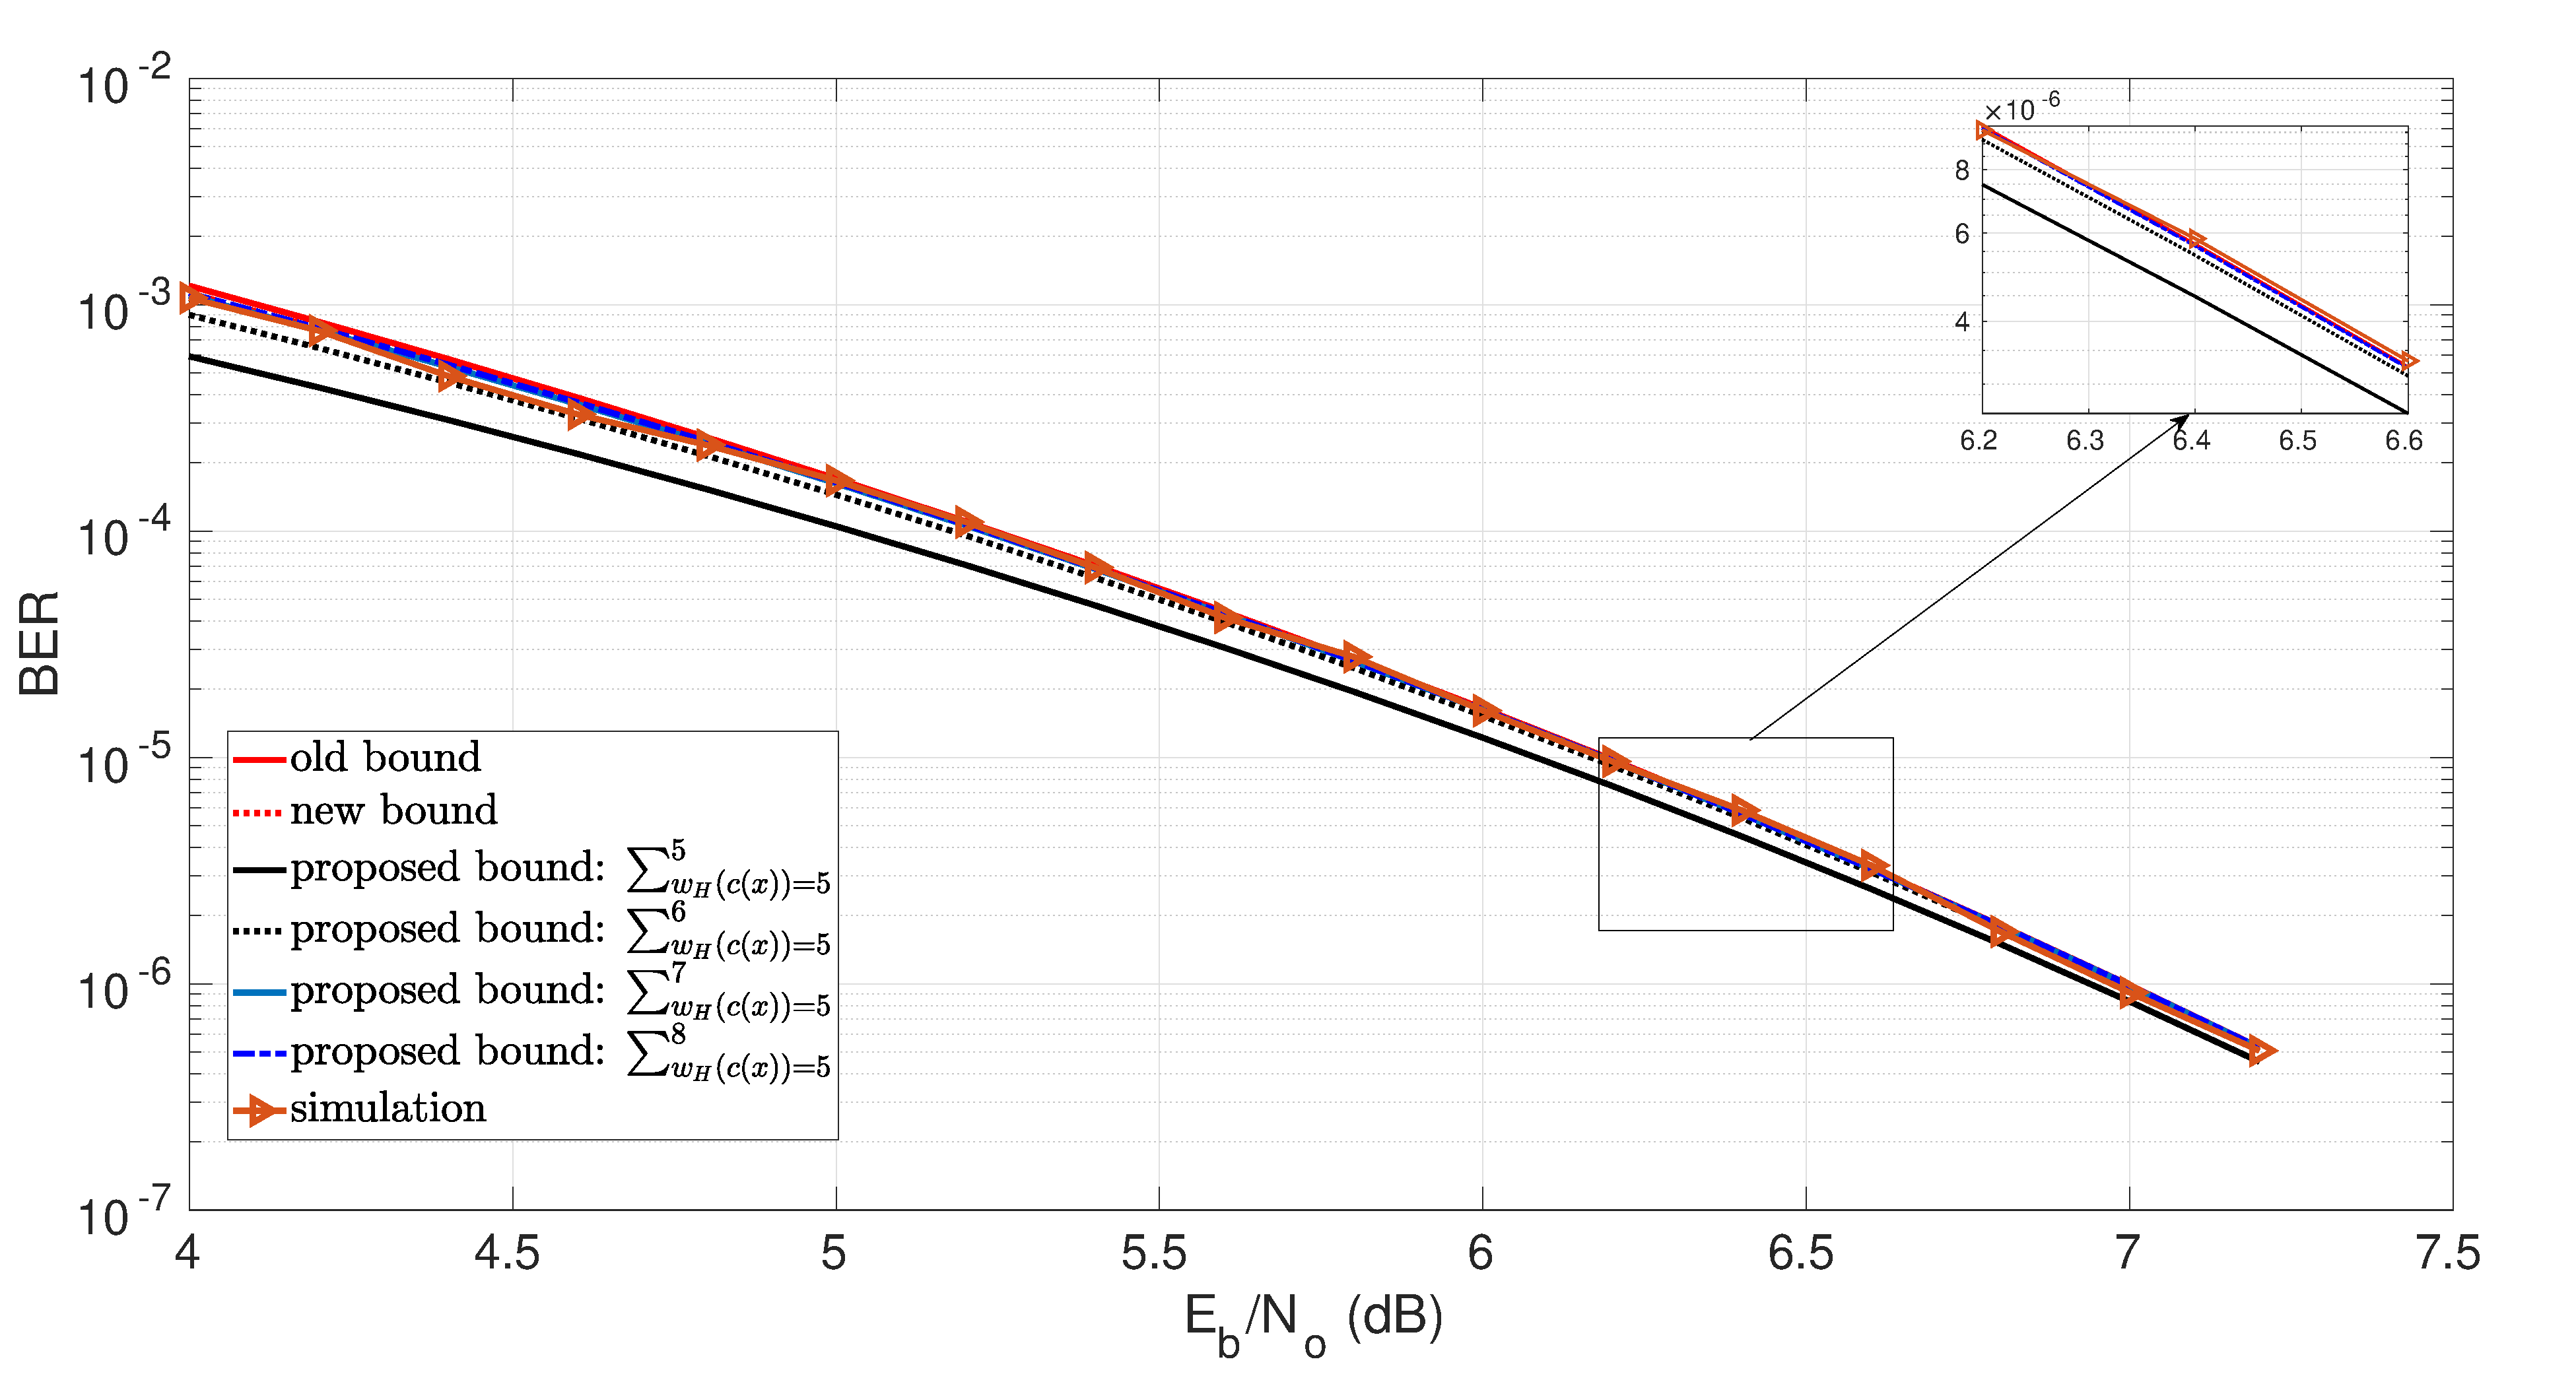
\includegraphics[width=1\textwidth]{./Images/RSC_5_7_lower_weights3.eps}
	\captionof{figure}{Old Bound vs New Bound vs Simulation for 5/7 RSC Code}
	\label{simFig1}
\end{figure}


\begin{figure}[htbp]
	\centering
	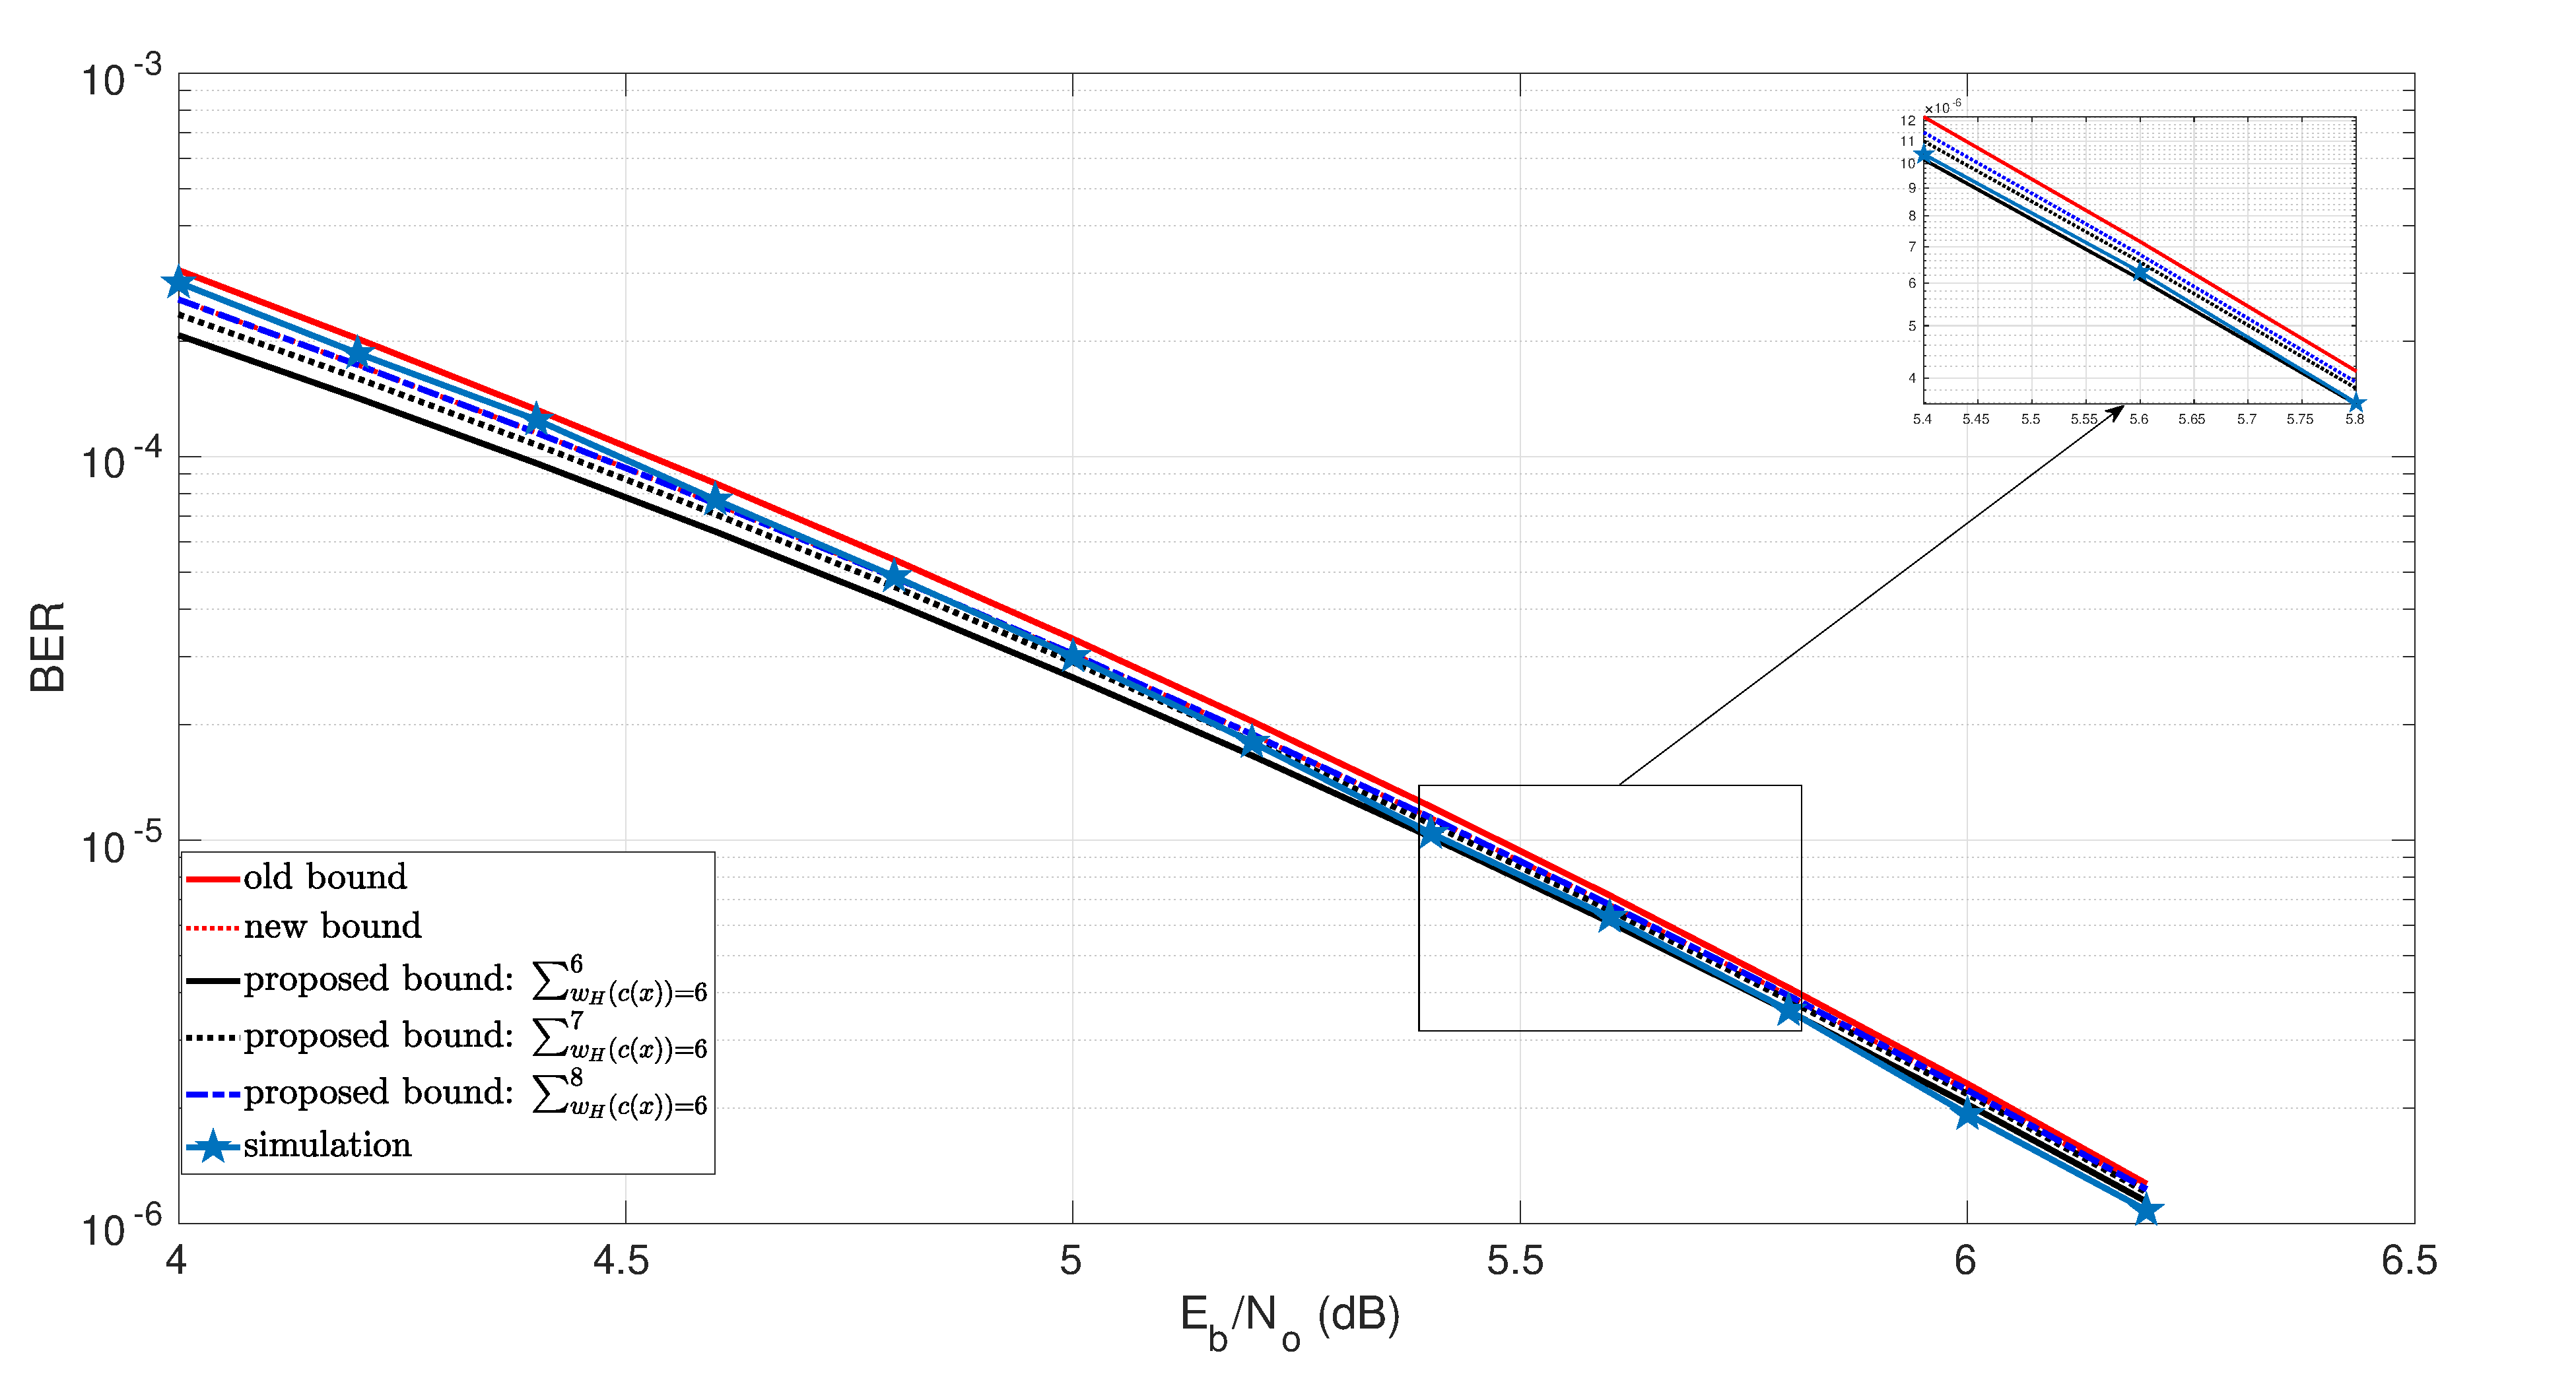
\includegraphics[width=1\textwidth]{./Images/RSC_37_21_lower_weights3.eps}
	\caption{Old Bound vs New Bound vs Simulation for 37/21 RSC Code}
	\label{simFig2}
\end{figure}


%Even though it is possible to improve the accuracy of our proposed bound by considering SCs and PCs of weight-4. 

\begin{figure}[htbp]
	\centering
	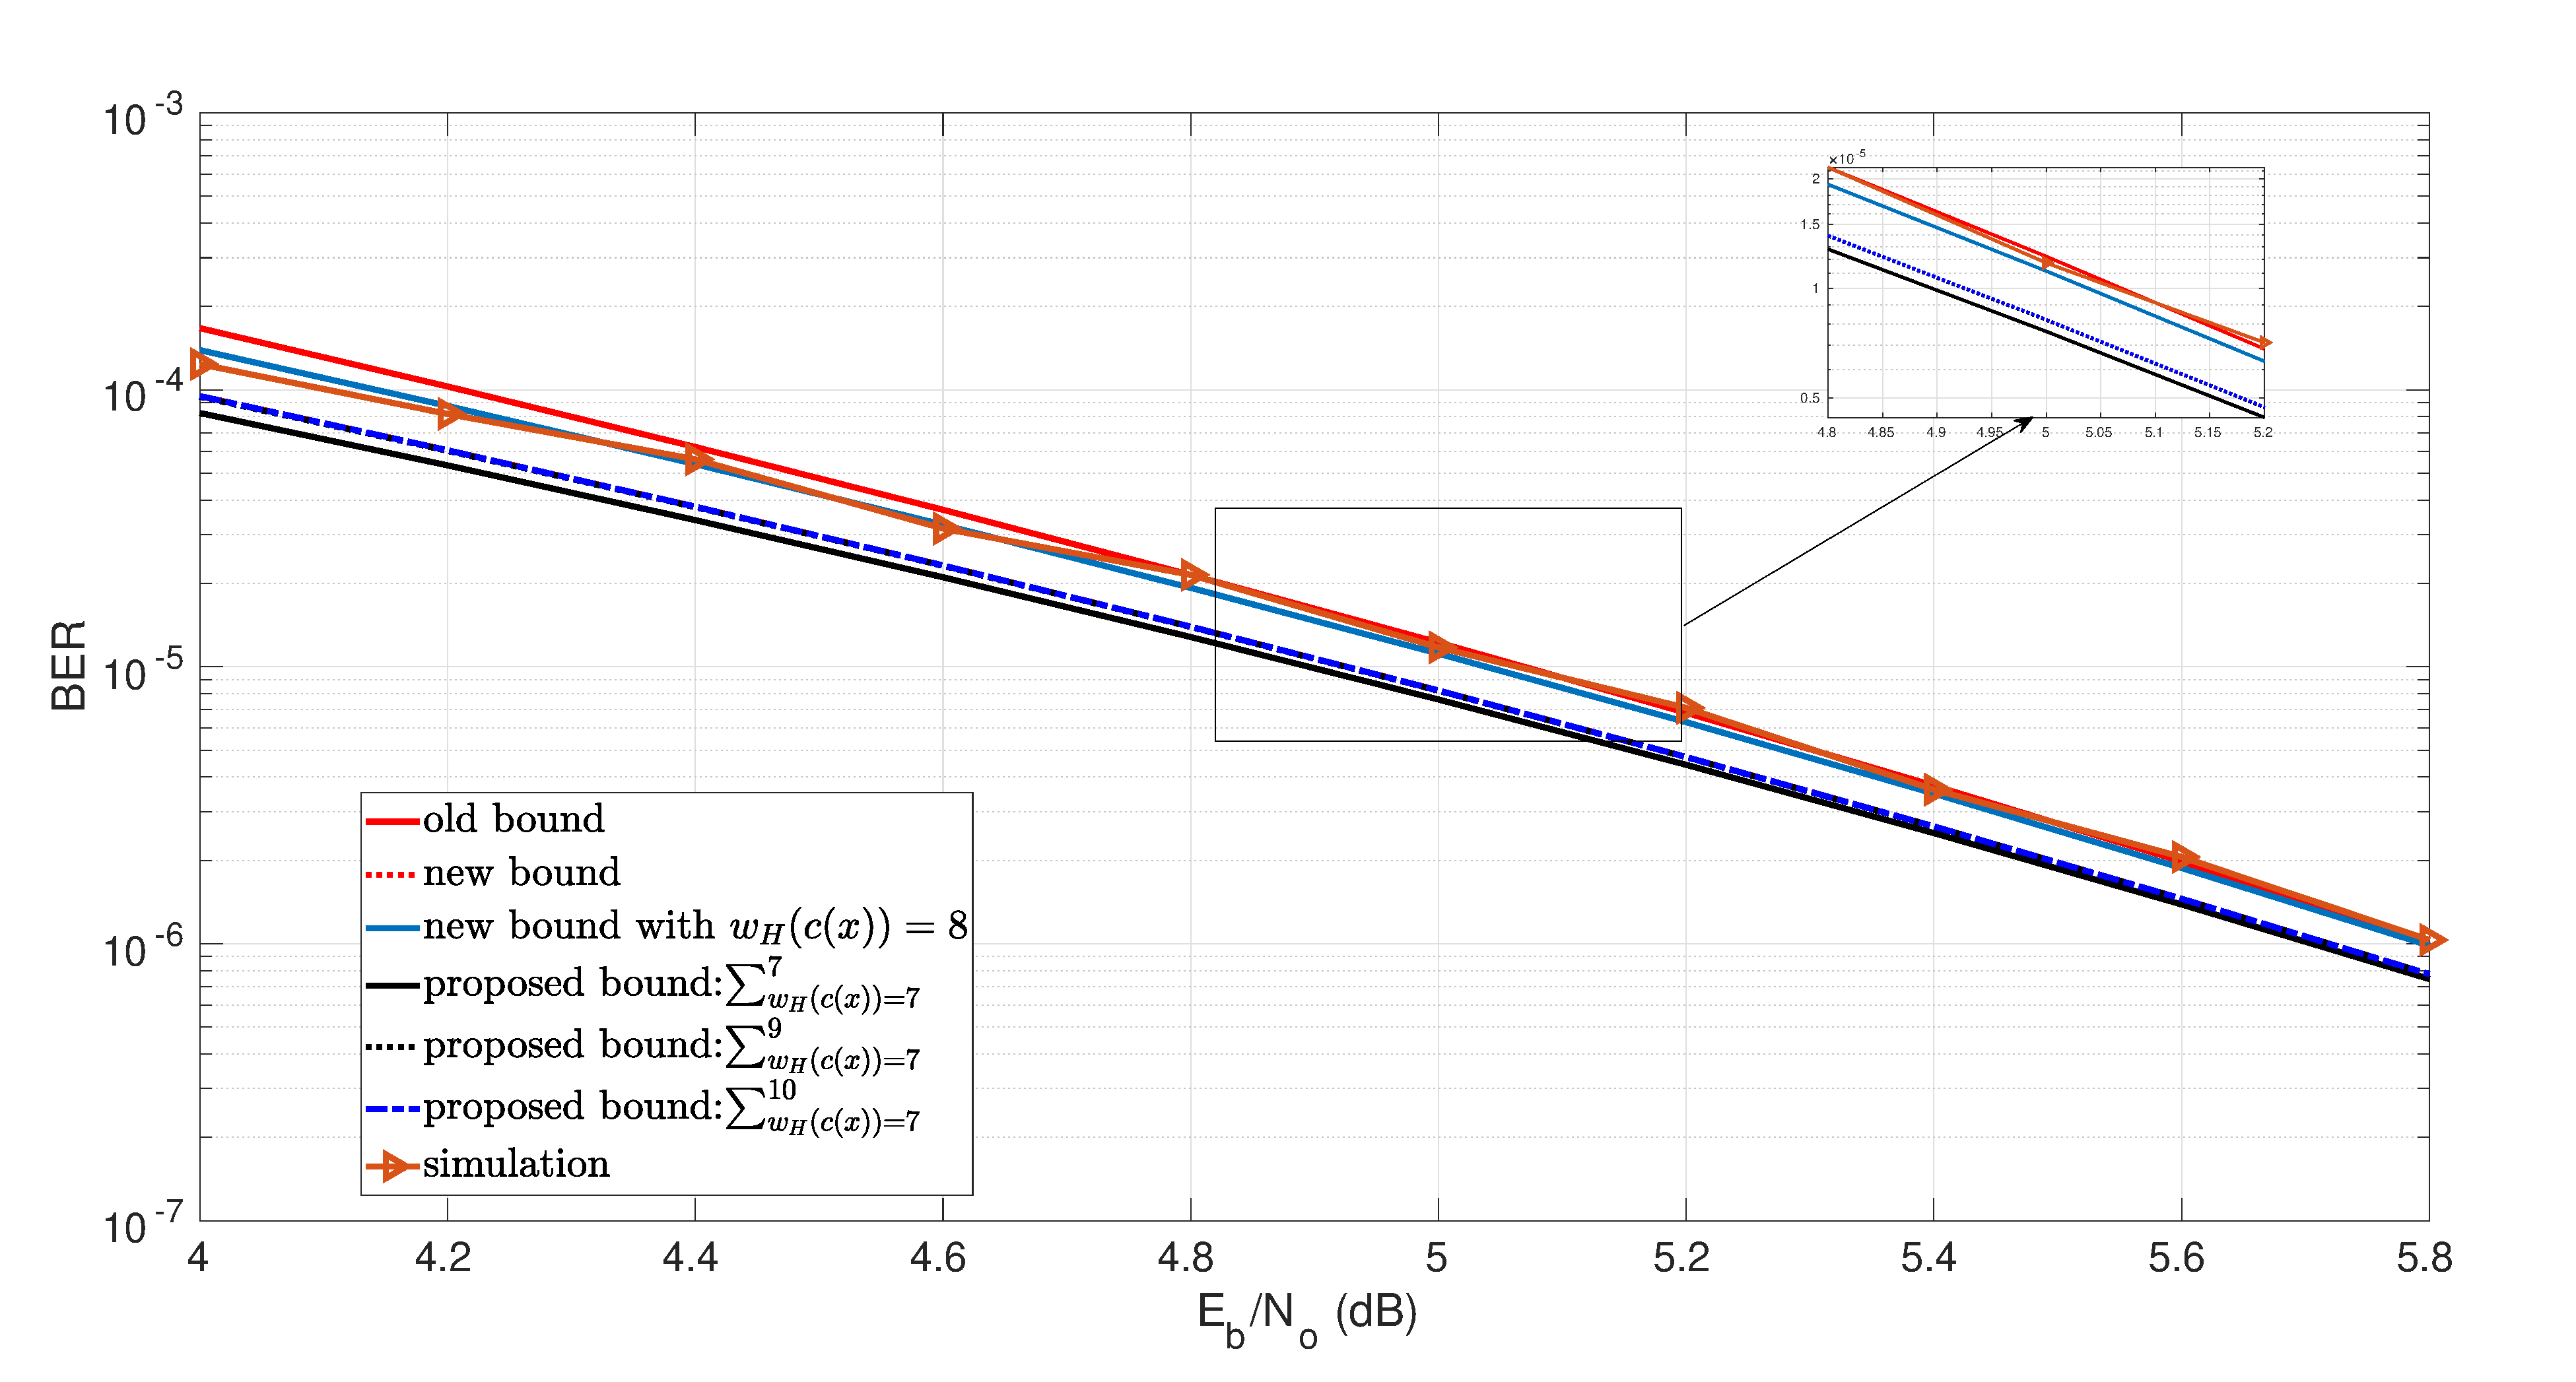
\includegraphics[width=1\textwidth]{./Images/RSC_23_35_lower_weights3.eps}
	\caption{Old Bound vs New Bound vs Simulation for 23/35 RSC Code}
	\label{simFig3}
\end{figure}

%\subsection{Discussion}
%
%We know from the previous discussion that take the codewords with weights $d_{\rm free}$ and $d_{\rm free +1}$ provides a good approximation of RSC code over AWGN channel. Now, we consider the code I-III from view point of interleaver design for Turbo code.
%
%For the code I, there 5 low-weight codewords 
%
%This means that when the 5/7 RSC code is used in a TC, the deterministic interleaver should be designed in such a way that it deals effectively with both weight-2 and weight-3 SCs. While, having to consider weight-3 SCs in the deterministic interleaver design introduces a bit of complexity, it is manageable since there is just a single $(m,n)$ pair that is associated with the weight-3 SCs.
%
%
%The fact that just a single $(m,n)$ pair needs to be considered for weight-3 SCs during interleaver design makes the 5/7 RSC code attractive for use in TCs.
%\label{ex-6}
%
%the added complexity as a result of considering weight-4 SCs in the interleaver design process makes this RSC code very unattractive for use in TCs.
%
%Given that weight-2 SCs and PCs are sufficient to derive the union bound, and deterministic interleaver design requires focusing on weight-2 SCs only, this RSC code is highly recommended for use in TCs.
%
%From Table \ref{novelTab15}, we observe that there are no weight-3 SCs. However, there exists weight-4 SCs that are not a combination of weight-2 SCs and when this RSC code is used in TCs, the deterministic interleaver needs to be designed to cater for weight-2 SCs as well as such weight-4 SCs. 




\newpage
%\section{Simulation and Theoretical Results}
\label{sec5}
In this section, we compare the bounds obtained via our novel method to bounds obtained using the transfer function method as well as the simulation results for the $5/7,~37/21$ and $23/35$ RSC codes, each with a frame size $N=64$. 
%For each RSC code and a frame size of $N=64$, the codeword is BPSK modulated and transmitted over the AWGN channel. At the receiver end, the Viterbi algorithm is used to decode before a decision is made on the decoded sequence.

We set $d_{\text{max}}=d_{\text{min}}+3$ and using our novel method outlined in the previous section,  we obtained the low-weight codeword component patterns for each RSC code and the results are shown in Tables \ref{novelTab13},  \ref{novelTab14} and \ref{novelTab15} respectively. We then calculate the lower bounds for our novel method and the transfer function using \eqref{novelEq7} and its original version in \cite{ref4} respectively. 
%It is worth noting that in all the tables, the codeword components are arranged in ascending order of codeword weight, with the $d_{\text{free}}$ components at the top of the table.  
%(quarantine)%For each RSC codeThese were obtained by dividing the general form of $h(x)$ for $w_H(\bh)=2$ and ($w_H(\bh)=2$ if it exists) by $f(x)$ and multiplying it by $g(x)$ to obtain $b(x)$ for a given RSC code. This process is repeated doing the same for the general form of $b(x)$. In both cases $a(x),~b(x)$ and $h(x)$ are only added to the list if $w_H(\bc) \leq d_{\text{max}}$.
\begin{table}[htbp]
 \caption{Partial Codeword Component Pattern Distance Spectrum for the $5/7$ RSC code, $d_{\text{free}}=5$}
\centering
 \begin{tabularx}{0.75\textwidth}{Xlll} 
 \hline
 $w_H(c(x))$& $a(x)$ & $b(x)$ & $h(x)$ \\ %[0.5ex] 
 \hline\hline
5&$1$ & $1+x+x^{2}$ & $1+x^2$\\
\hline\hline
6&$1+x^2$ & $1+x+x^3+x^4$ & $1+x^{4}$\\
%\hline
&$1+x$ & $1+x^3$ & $1+x+x^2+x^3$\\
\hline\hline
&$1+x^2+x^4$ & $1+x+x^3+x^5+x^6$ & $1+x^{6}$\\
%\hline\hline
7&$1+x^2+x^3$ & $1+x+x^5$ & $1+x^3+x^4+x^5$\\
%\hline
&$1+x+x^2$ & $1+x^2+x^4$ & $1+x+x^3+x^4$\\
%\hline
&$1+x+x^3$ & $1+x^4+x^5$ & $1+x+x^2+x^5$\\
\hline \hline
8&$1+x^2+x^4+x^6$ & $1+x+x^3+x^5+x^7+x^8$ & $1+x^8$\\
%\hline
&$1+x+x^3+x^4$ & $1+x^6$ & $1+x+x^2+x^4+x^5+x^6$\\
\hline
%======extra
%\hline
%$1+x+x^3+x^5$ & $1+x^4+x^6+x^7$ & $1+x+x^2+x^7$\\
%\hline
%$1+x+x^2+x^4$ & $1+x^2+x^5+x^6$ & $1+x+x^3+x^6$\\
%\hline
%$1+x+x^2+x^3$ & $1+x^2+x^3+x^5$ & $1+x+x^4+x^5$\\
%\hline
%$1+x^2+x^3+x^5$ & $1+x+x^6+x^7$ & $1+x^3+x^4+x^7$\\
%\hline
%$1+x^2+x^3+x^4$ & $1+x+x^4+x^6$ & $1+x^3+x^5+x^6$\\
%\hline
%$1+x^2+x^4+x^5$ & $1+x+x^3+x^7$ & $1+x^5+x^6+x^7$\\
 \end{tabularx}
 
 \label{novelTab13}
\end{table}

\begin{figure}[htbp]
\centering
		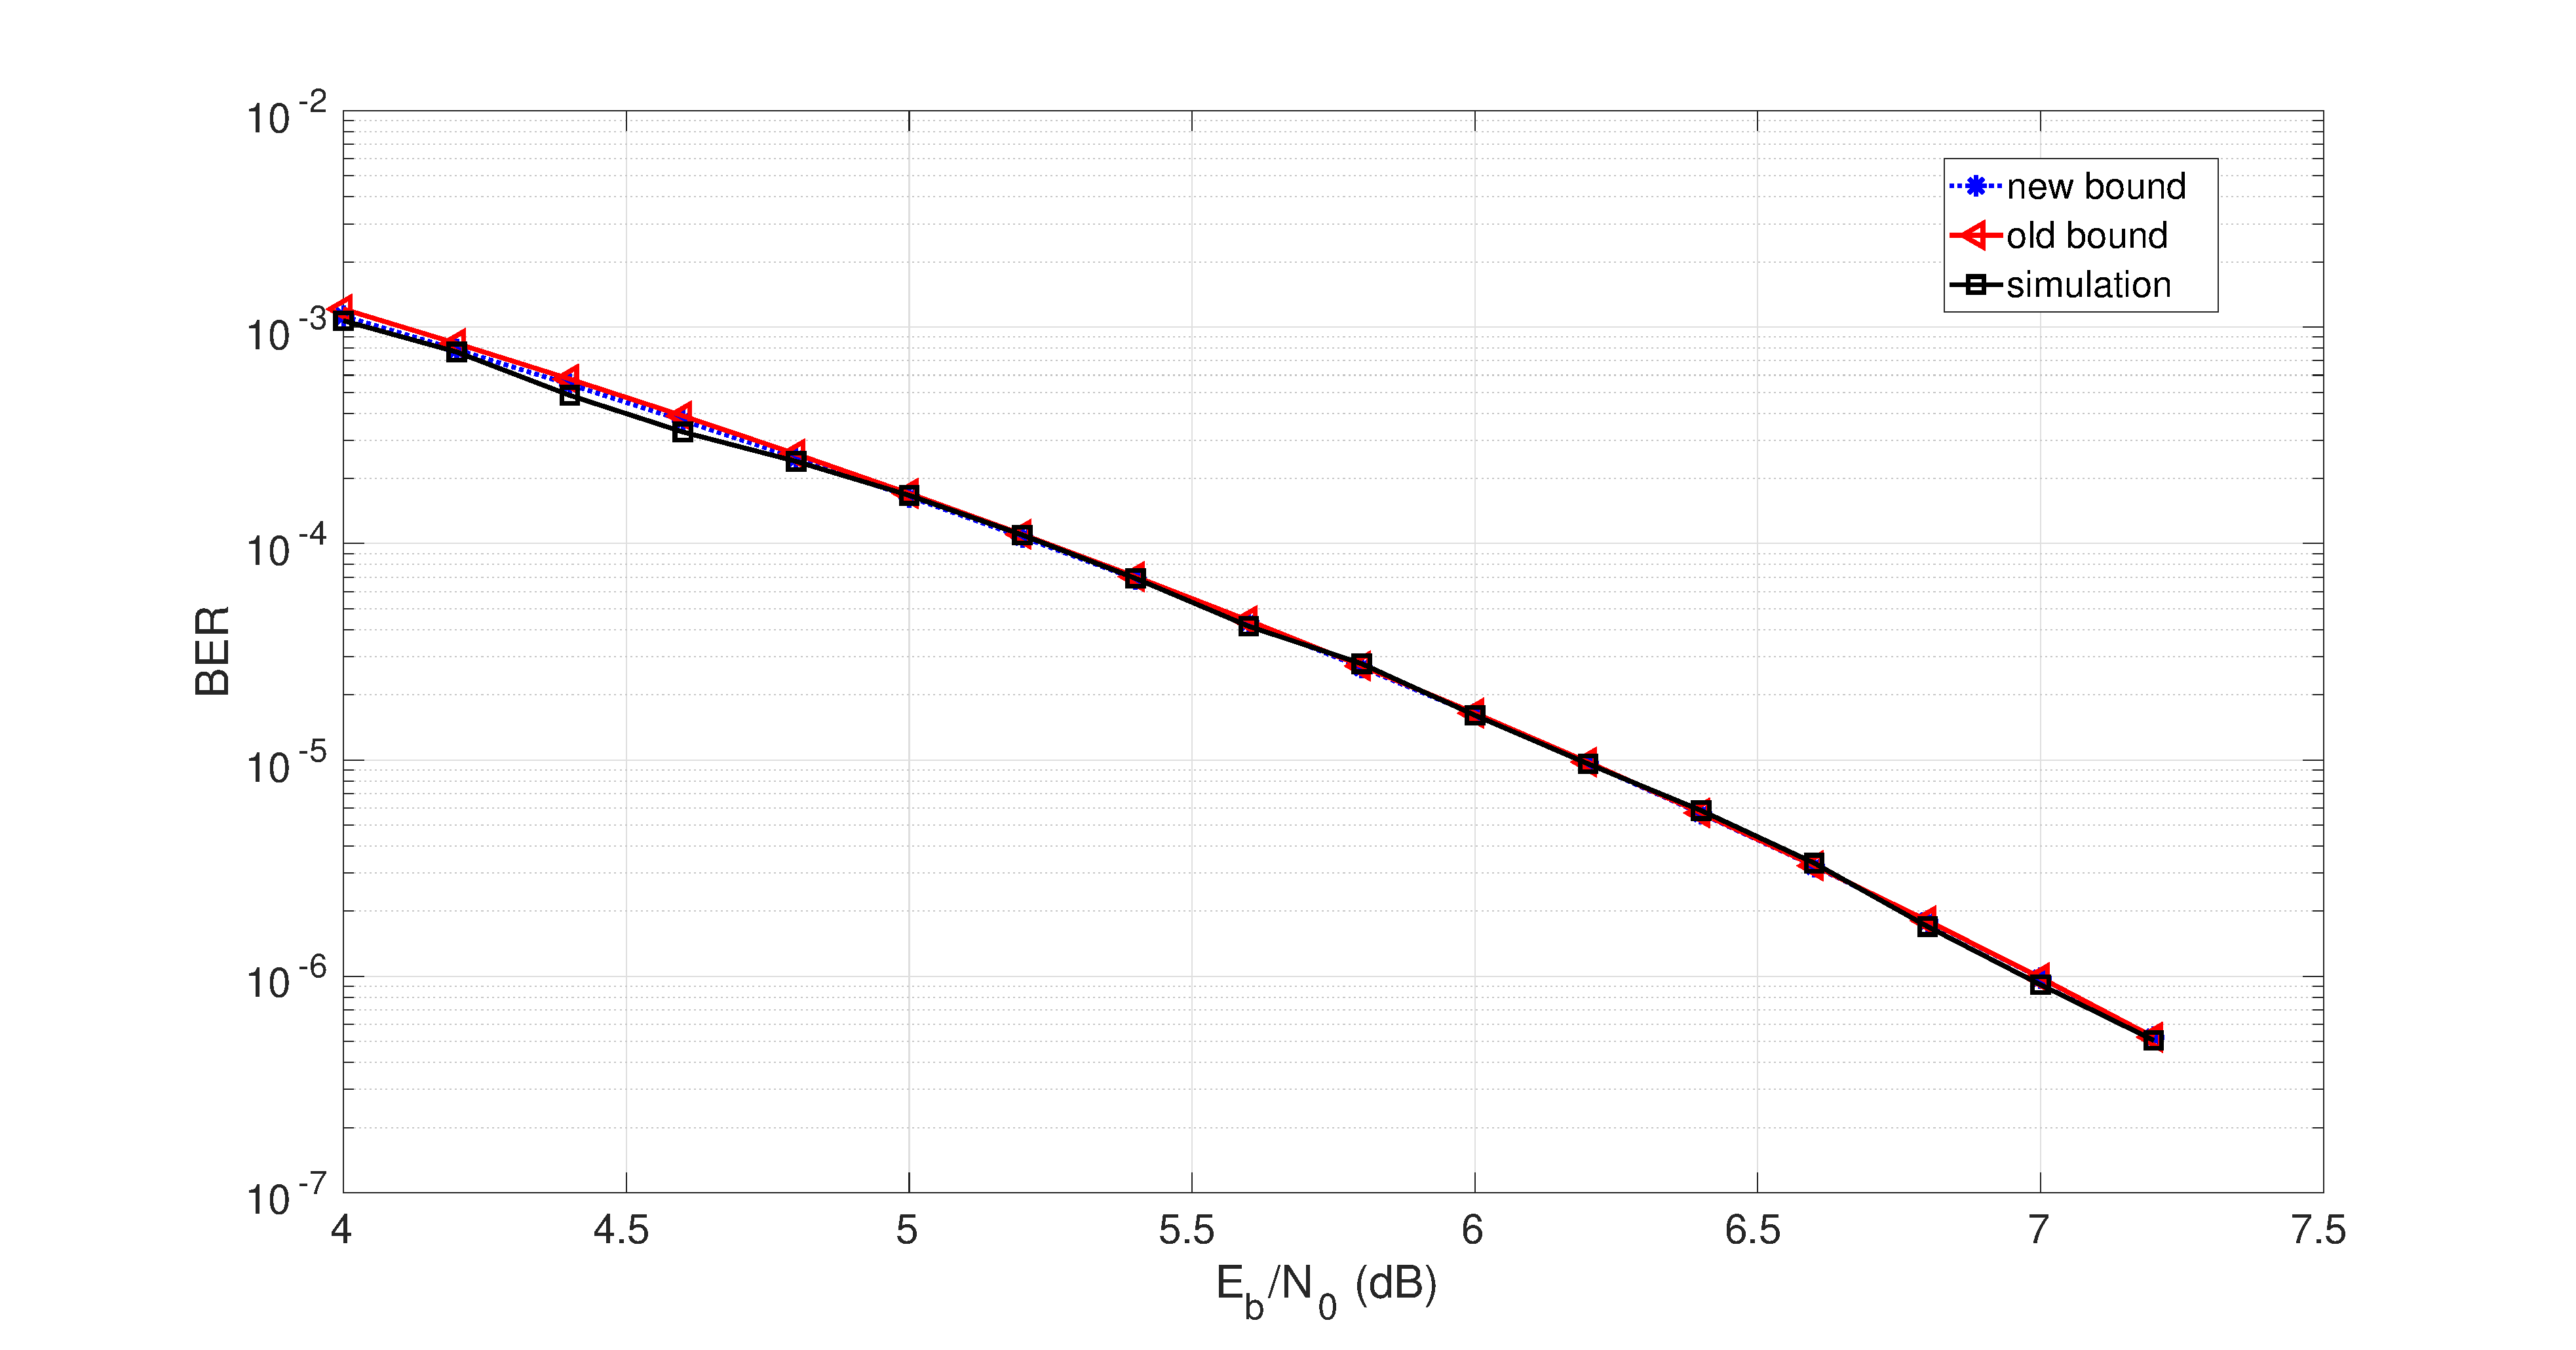
\includegraphics[width=0.5\textwidth]{./Images/RSC_5_7_lower_weights.eps}
		\captionof{figure}{Old Bound vs New Bound vs Simulation for 5/7 RSC Code}
		\label{simFig1}
		\end{figure}
		
Fig. \ref{simFig1} shows the simulation results for the $5/7$ RSC code as well as the lower bounds obtained using the transfer function as well as our novel method. The feedforward connection has the polynomial representation $1+x^2$ and can be factorized into the irreducible polynomial $1+x$. From Example \ref{ex-3}, we observe that whiles there exists weight-2 PCs, there  are no weight-3 PCs for $1+x^2$
The feedback connection has the polynomial representation $1+x+x^2$, which is an irreducuble polynomial and from Example \ref{ex-1}, we can confirm that there exists weight-2 SCs as well as weight-3 SCs. In Fig. \ref{simFig1}, we observe that there is some difference between the new (novel method) bound and the old (transfer function) bound, but they tend to converge as $E_b/N_0$ increases. This suggests that the approximation $ \bigcup_{d = d_{\text{min}}}^{d_{\text{max}}} \cA'_c(d) $ used in our novel method is sufficient for the $5/7$ RSC code.

%We observe that for both Fig. \ref{simFig1} and Fig. \ref{simFig2}, there is some difference between the new (novel method) bound and the old (transfer function) bound, but they tend to converge as $E_b/N_0$ increases. This suggests that the approximation used with our novel method is sufficient for these RSC codes.

%codewords generated considering $b(x),~w_H(b(x))>3$ as well as codewords which have a parity-check sequence $h(x),~w_H(h(x))>3$ do not have much effect on the BER of the code as $E_b/N_0$ increases.

%The gap that is observed in the low $E_b/N_0$ regions is attributed to omitting codewords generated by the RTZ inputs of weight $w_H(\bb)=4$ as well as codewords with parity-check sequences $w_H(\bh)=4$ in our calculation of the new bound. 

%Fig. \ref{simFig4} and Fig. \ref{simFig5} are similar to  Fig. \ref{simFig1} and Fig. \ref{simFig2}, with the only difference being that codewords generated by the RTZ inputs of weight $w_H(\bb)=4$ as well as codewords with parity-check sequences $w_H(\bh)=4$ have been added in our calculation of the new bound. The new and old bounds match up and the accuracy of our bound is greatly improved.The simulation results also agree with the bounds as they also converge with the bounds.

\begin{table}[htbp]
 \caption{Partial Codeword Component Pattern Distance Spectrum for the $37/21$ RSC code, $d_{\text{free}}=6$}
\centering
 \begin{tabularx}{0.75\textwidth}{Xlll} 
 \hline
 $w_H(c(x))$&$a(x)$ & $b(x)$ & $h(x)$ \\ [0.5ex] 
 \hline\hline
6&$1+x$ & $1+x+x^{4}+x^5$ & $1+x^5$\\
\hline\hline
7&$1$ & $1+x^4$ & $1+x+x^2+x^3+x^4$\\
\hline\hline
8&$1+x+x^5+x^6$ & $1+x+x^4+x^6+x^9+x^{10}$ & $1+x^{10}$\\
\hline
%$1+x+x^4+x^5$ & $1+x+x^8+x^9$ & $1+x^4+x^5+x^9$\\
%\hline
%$1+x^2$ & $1+x^2+x^4+x^6$ & $1+x+x^5+x^6$\\
%\hline
%$1+x+x^5$ & $1+x+x^4+x^9$ & $1+x^6+x^7+x^8+x^9$\\
%\hline
%$1+x+x^4$ & $1+x+x^5+x^8$ & $1+x^4+x^6+x^7+x^8$\\
%\hline
%$1+x^2+x^4$ & $1+x^2+x^6+x^8$ & $1+x+x^4+x^7+x^8$\\
%\hline
%$1+x^3+x^4$& $1+x^3+x^7+x^8$ & $1+x+x^2+x^4+x^8$\\
%\hline
%$1+x^4+x^5$ & $1+x^5+x^8+x^9$ & $1+x+x^2+x^3+x^9$\\
 \end{tabularx}
 
 \label{novelTab14}
\end{table}

\begin{figure}[htbp]
\centering
		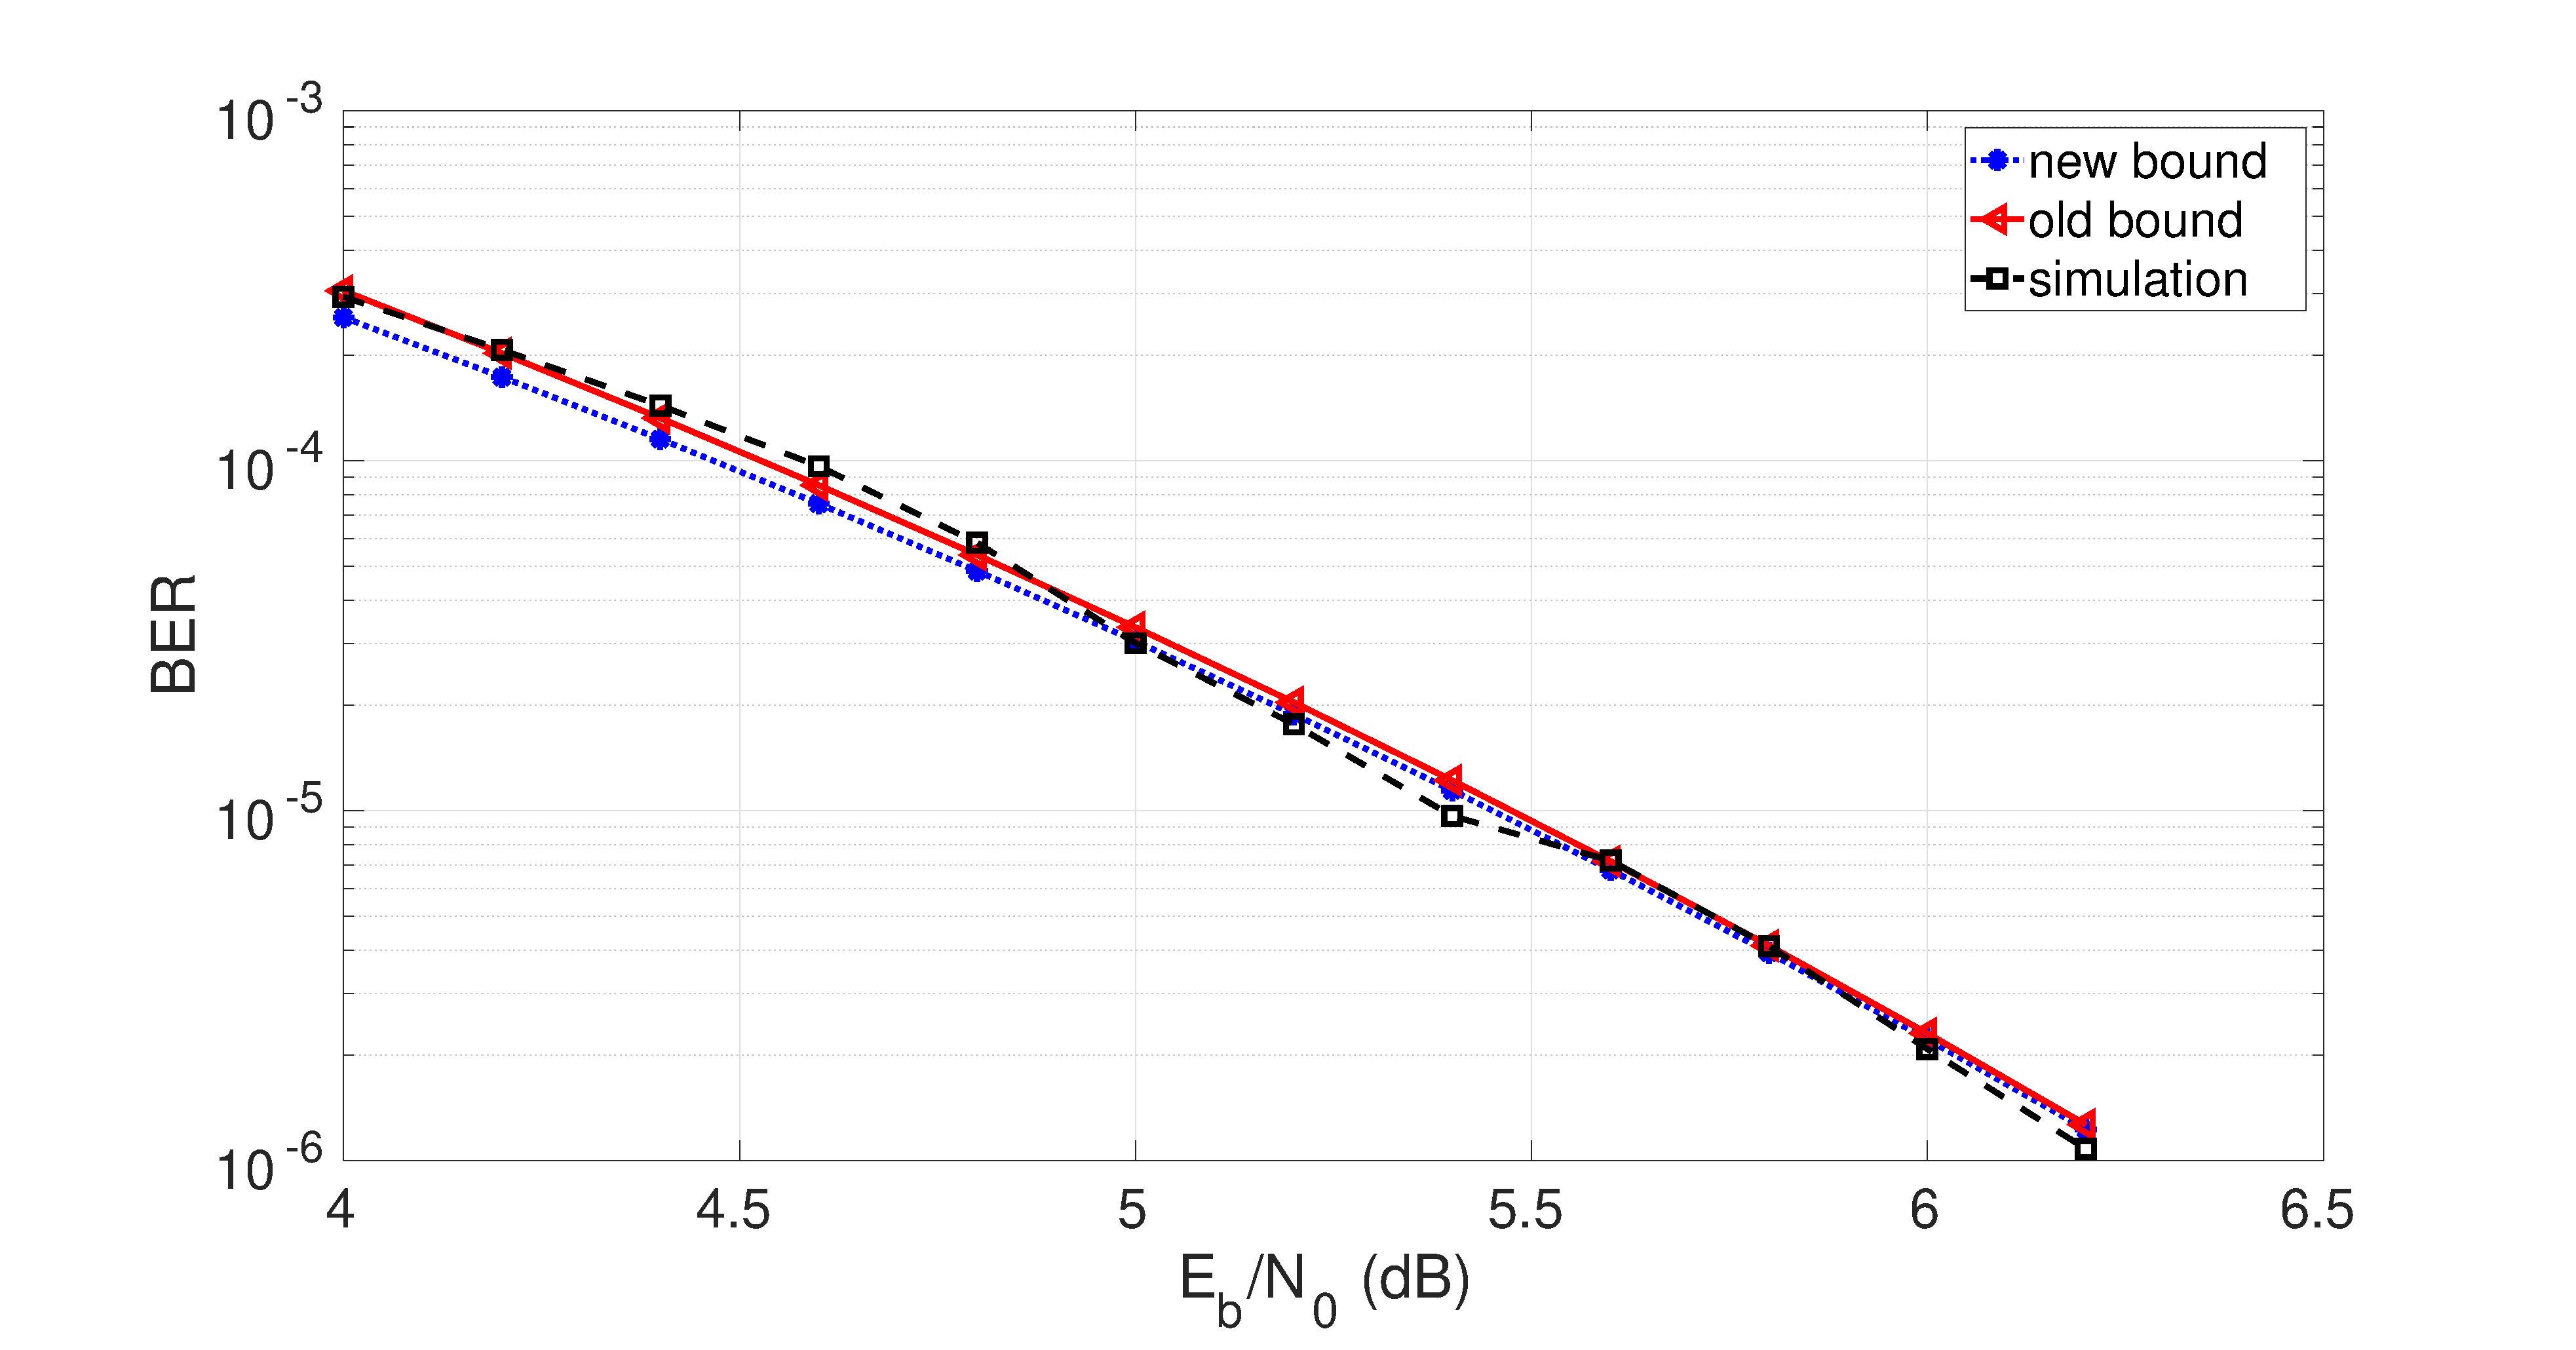
\includegraphics[width=0.5\textwidth]{./Images/RSC_37_21_lower_weights.eps}
		\caption{Old Bound vs New Bound vs Simulation for 37/21 RSC Code}
		\label{simFig2}
		\end{figure}
Fig. \ref{simFig2} shows the simulation results for the $37/21$ RSC code as well as the lower bounds obtained using the transfer function as well as our novel method. The feedforward connection has the polynomial representation $1+x+x^2+x^3+x^4$, which is an irreducible polynomial. From Example \ref{ex-2}, we confirm that whiles weight-2 PCs exist, there are no wight-3 PCs. The feedback connection has the polynomial representation $1+x^4$, and from Example \ref{ex-3}, we can deduce that weight-2 SCs exist, but there are no weight-3 SCs. In Fig. \ref{simFig2}, we observe that there is some difference between the new (novel method) bound and the old (transfer function) bound, but they tend to converge as $E_b/N_0$ increases. This suggests that the approximation $ \bigcup_{d = d_{\text{min}}}^{d_{\text{max}}} \cA'_c(d) $ used in our novel method is also sufficient for the $37/21$ RSC code.
%In \ref{simFig3}, we observe that the old bounds and simulation results converge as the Eb/No value increases. However, there is a very distinct gap between the new bound and the old bound. Moreover, the bounds do not converge as the Eb/No increases. This suggests that the approximation used in our novel method is insufficient for this RSC code and considering  $w_H(h(x)),~w_H(b(x))=4$ might yield a more accurate bound.

\begin{table}[htbp]
 \caption{Partial Codeword Component Pattern Distance Spectrum for the $23/35$ RSC code, $d_{\text{free}}=7$}
\centering
\begin{tabularx}{0.75\textwidth}{lXlX} 
 \hline
$w_H(c(x))$ & $a(x)$ & $b(x)$ & $h(x)$ \\ [0.5ex] 
 \hline\hline
7&$1+x^2+x^3$ & $1+x^7$ & $1+x+x^2+x^6+x^7$\\
\hline
&$1$ & $1+x^2+x^3+x^4$ & $1+x+x^{4}$\\
\hline \hline
8&$1+x+x^2+x^3+x^5$ & $1+x^3+x^4+x^8+x^9$ & $1+x^7+x^9$\\
\hline\hline
9&$1+x+x^2+x^3+x^5+x^7+x^8$ & $1+x+x^3+x^4+x^7+x^{12}$ & $1+x^{11}+x^{12}$\\
\hline\hline
10&$1+x^2+x^3+x^7+x^9+x^{10}$ & $1+x^{14}$ & $1+x+x^2+x^6+x^8+x^9+x^{13}+x^{14}$\\
\hline
 \end{tabularx}
 
 \label{novelTab15}
\end{table}

\begin{figure}[htbp]
\centering
		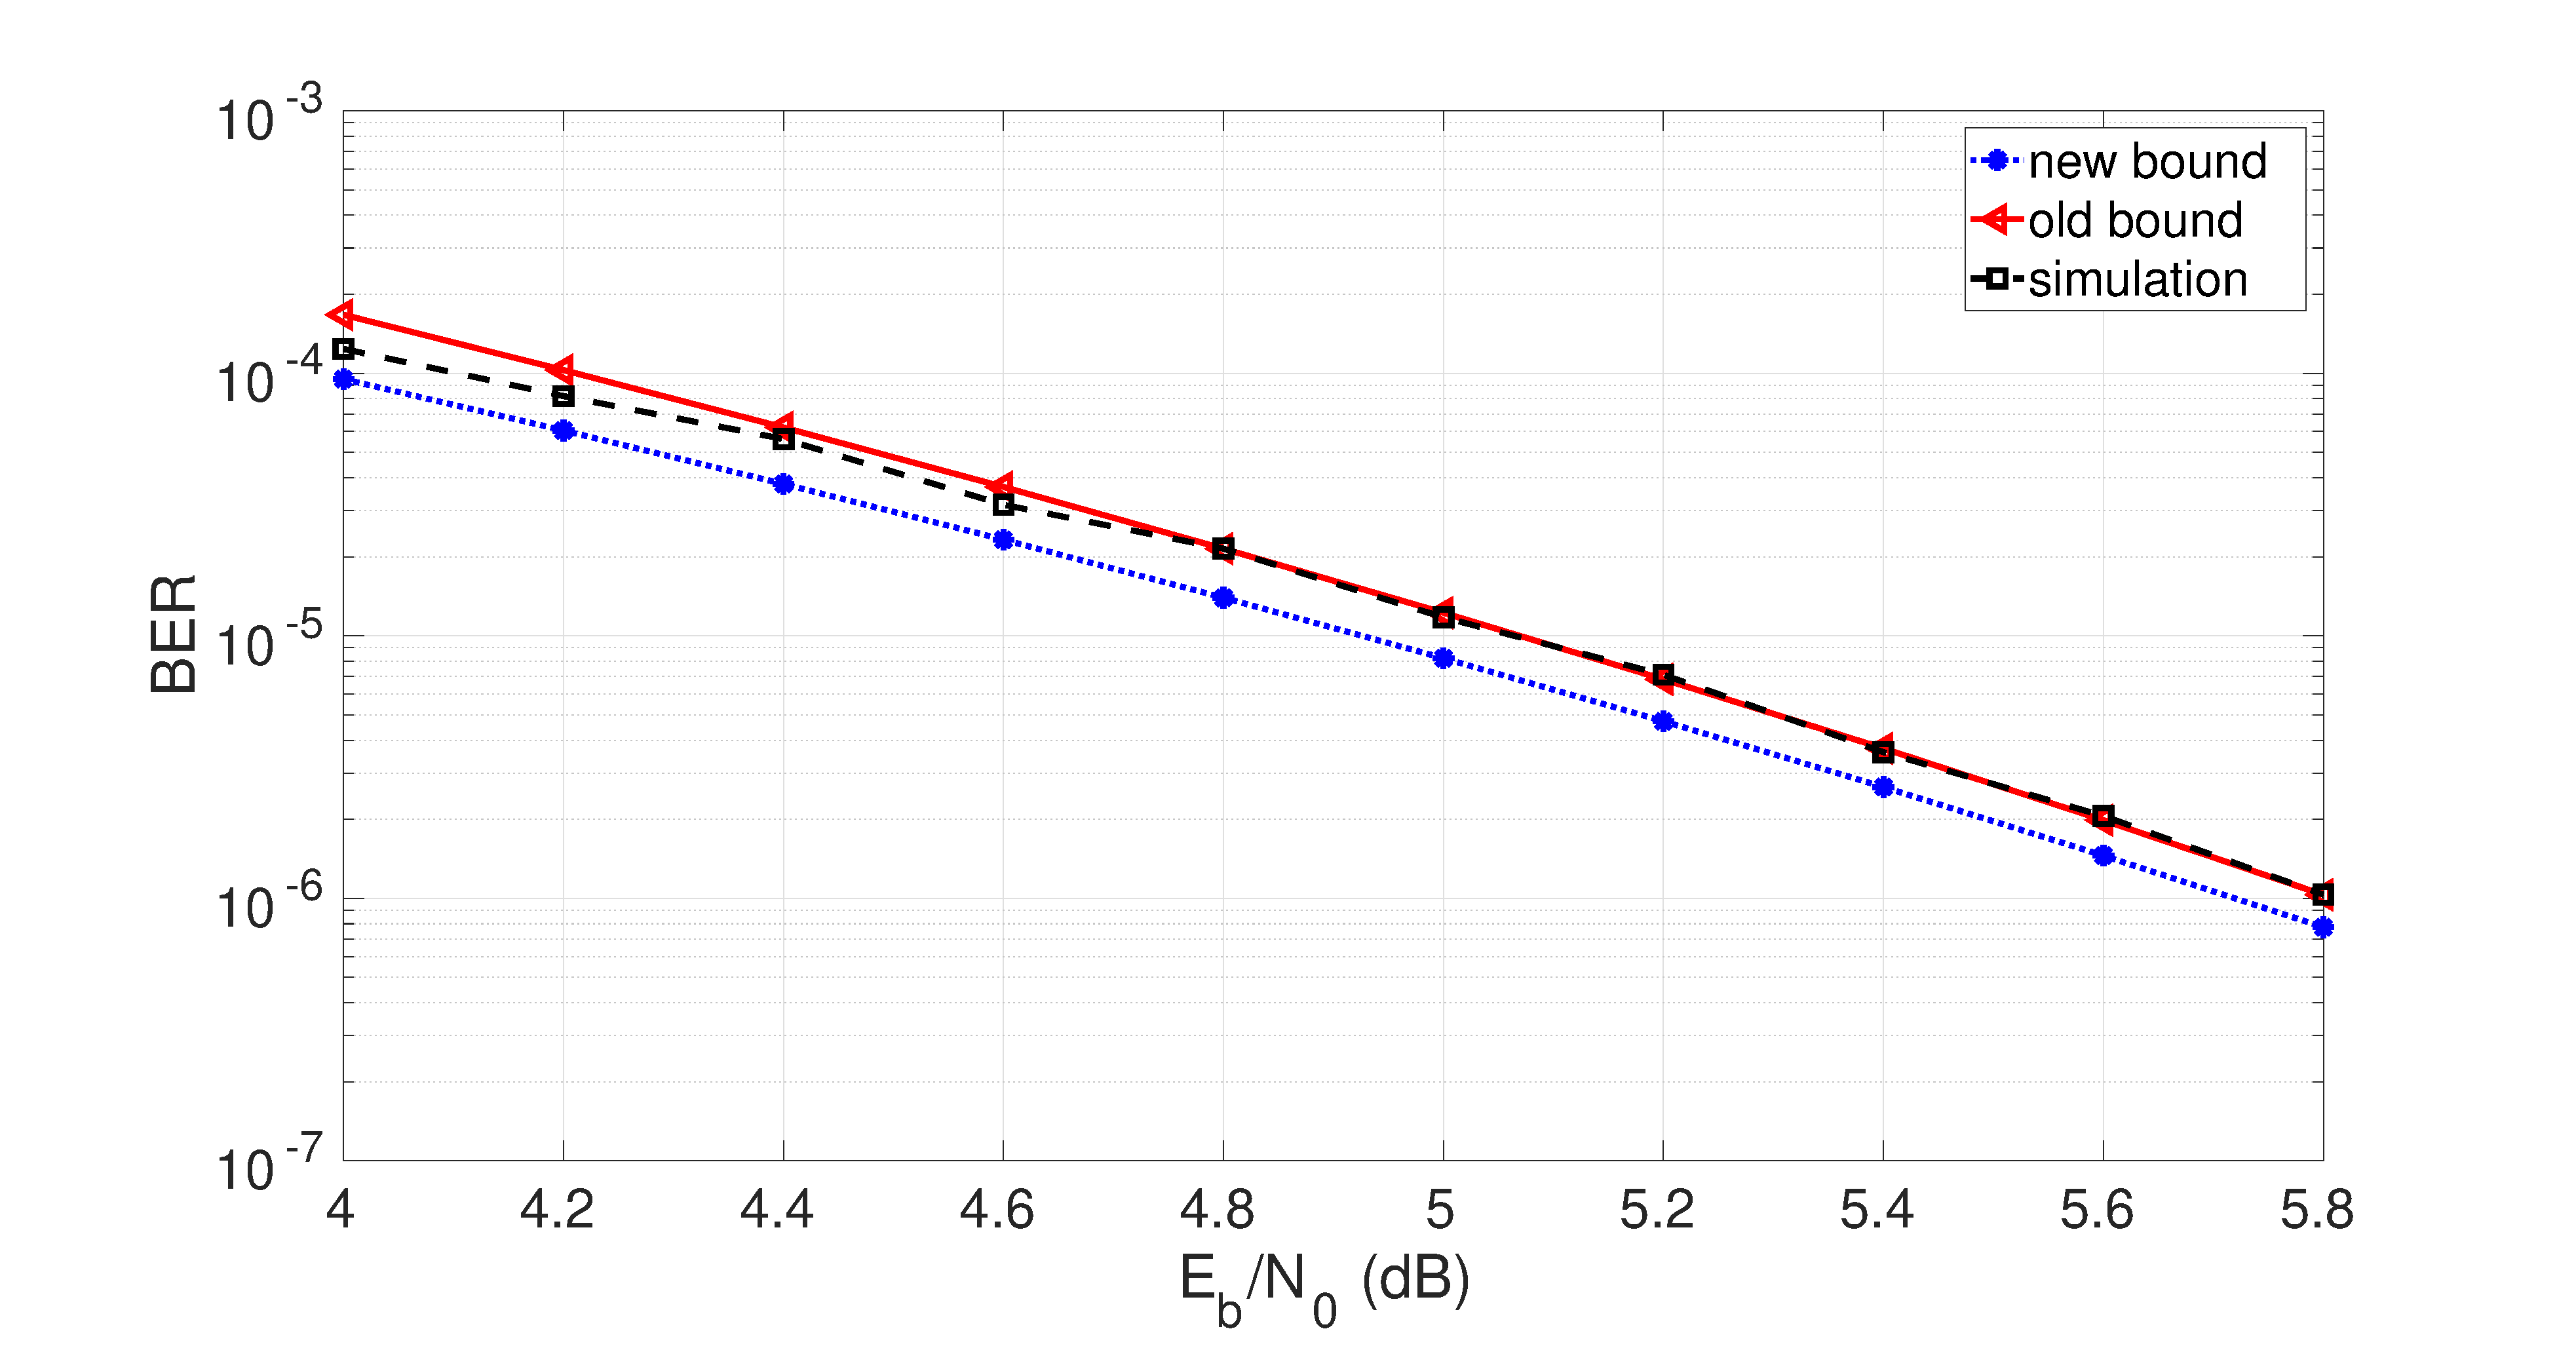
\includegraphics[width=0.5\textwidth]{./Images/RSC_23_35_lower_weights.eps}
		\caption{Old Bound vs New Bound vs Simulation for 23/35 RSC Code}
		\label{simFig3}
		\end{figure}
Fig. \ref{simFig3} shows the simulation results for the $23/35$ RSC code as well as the lower bounds obtained using the transfer function as well as our novel method. The feedforward connection has the polynomial representation $1+x+x^4$, which is similar in characteristic to the polynomial in Example \ref{ex-1}. It can easily be confirmed that there exists weight-2 and weight-3 PCs. For the weight-2 PCs, the general form for $a(x)$ is
\begin{equation*}
a(x)=\sum_{\ell=0}^{L-1} x^{15\ell}(1+x+x^{2}+x^3+x^5+x^7+x^8+x^{11})
\end{equation*}
and since it yields codewords such that $w_H(c(x))>d_{\text{max}}$, there are not included in our approximation of the lower bound, as can be observed from Table \ref{novelTab14}. The feedback connection has the polynomial representation $1+x^2+x^3+x^4$, which can be factorized into $2$ irreducible polynomials and it can easily be confirmed that there exists no weight-3 SCs, since $1+x$ is a factor. In Fig. \ref{simFig3}, we observe that the old (transfer function) bounds and simulation results converge as the $E_b/N_0$ value increases. However, there is some difference between the new (novel method) bound and the old (transfer function) bound, even as $E_b/N_0$ increases. This suggests that the approximation used in our novel method is insufficient for this $23/35$ RSC code and considering  $w_H(h(x)),~w_H(b(x))=4$ might yield a more accurate bound.


%\begin{figure}[h!]
%\centering
%		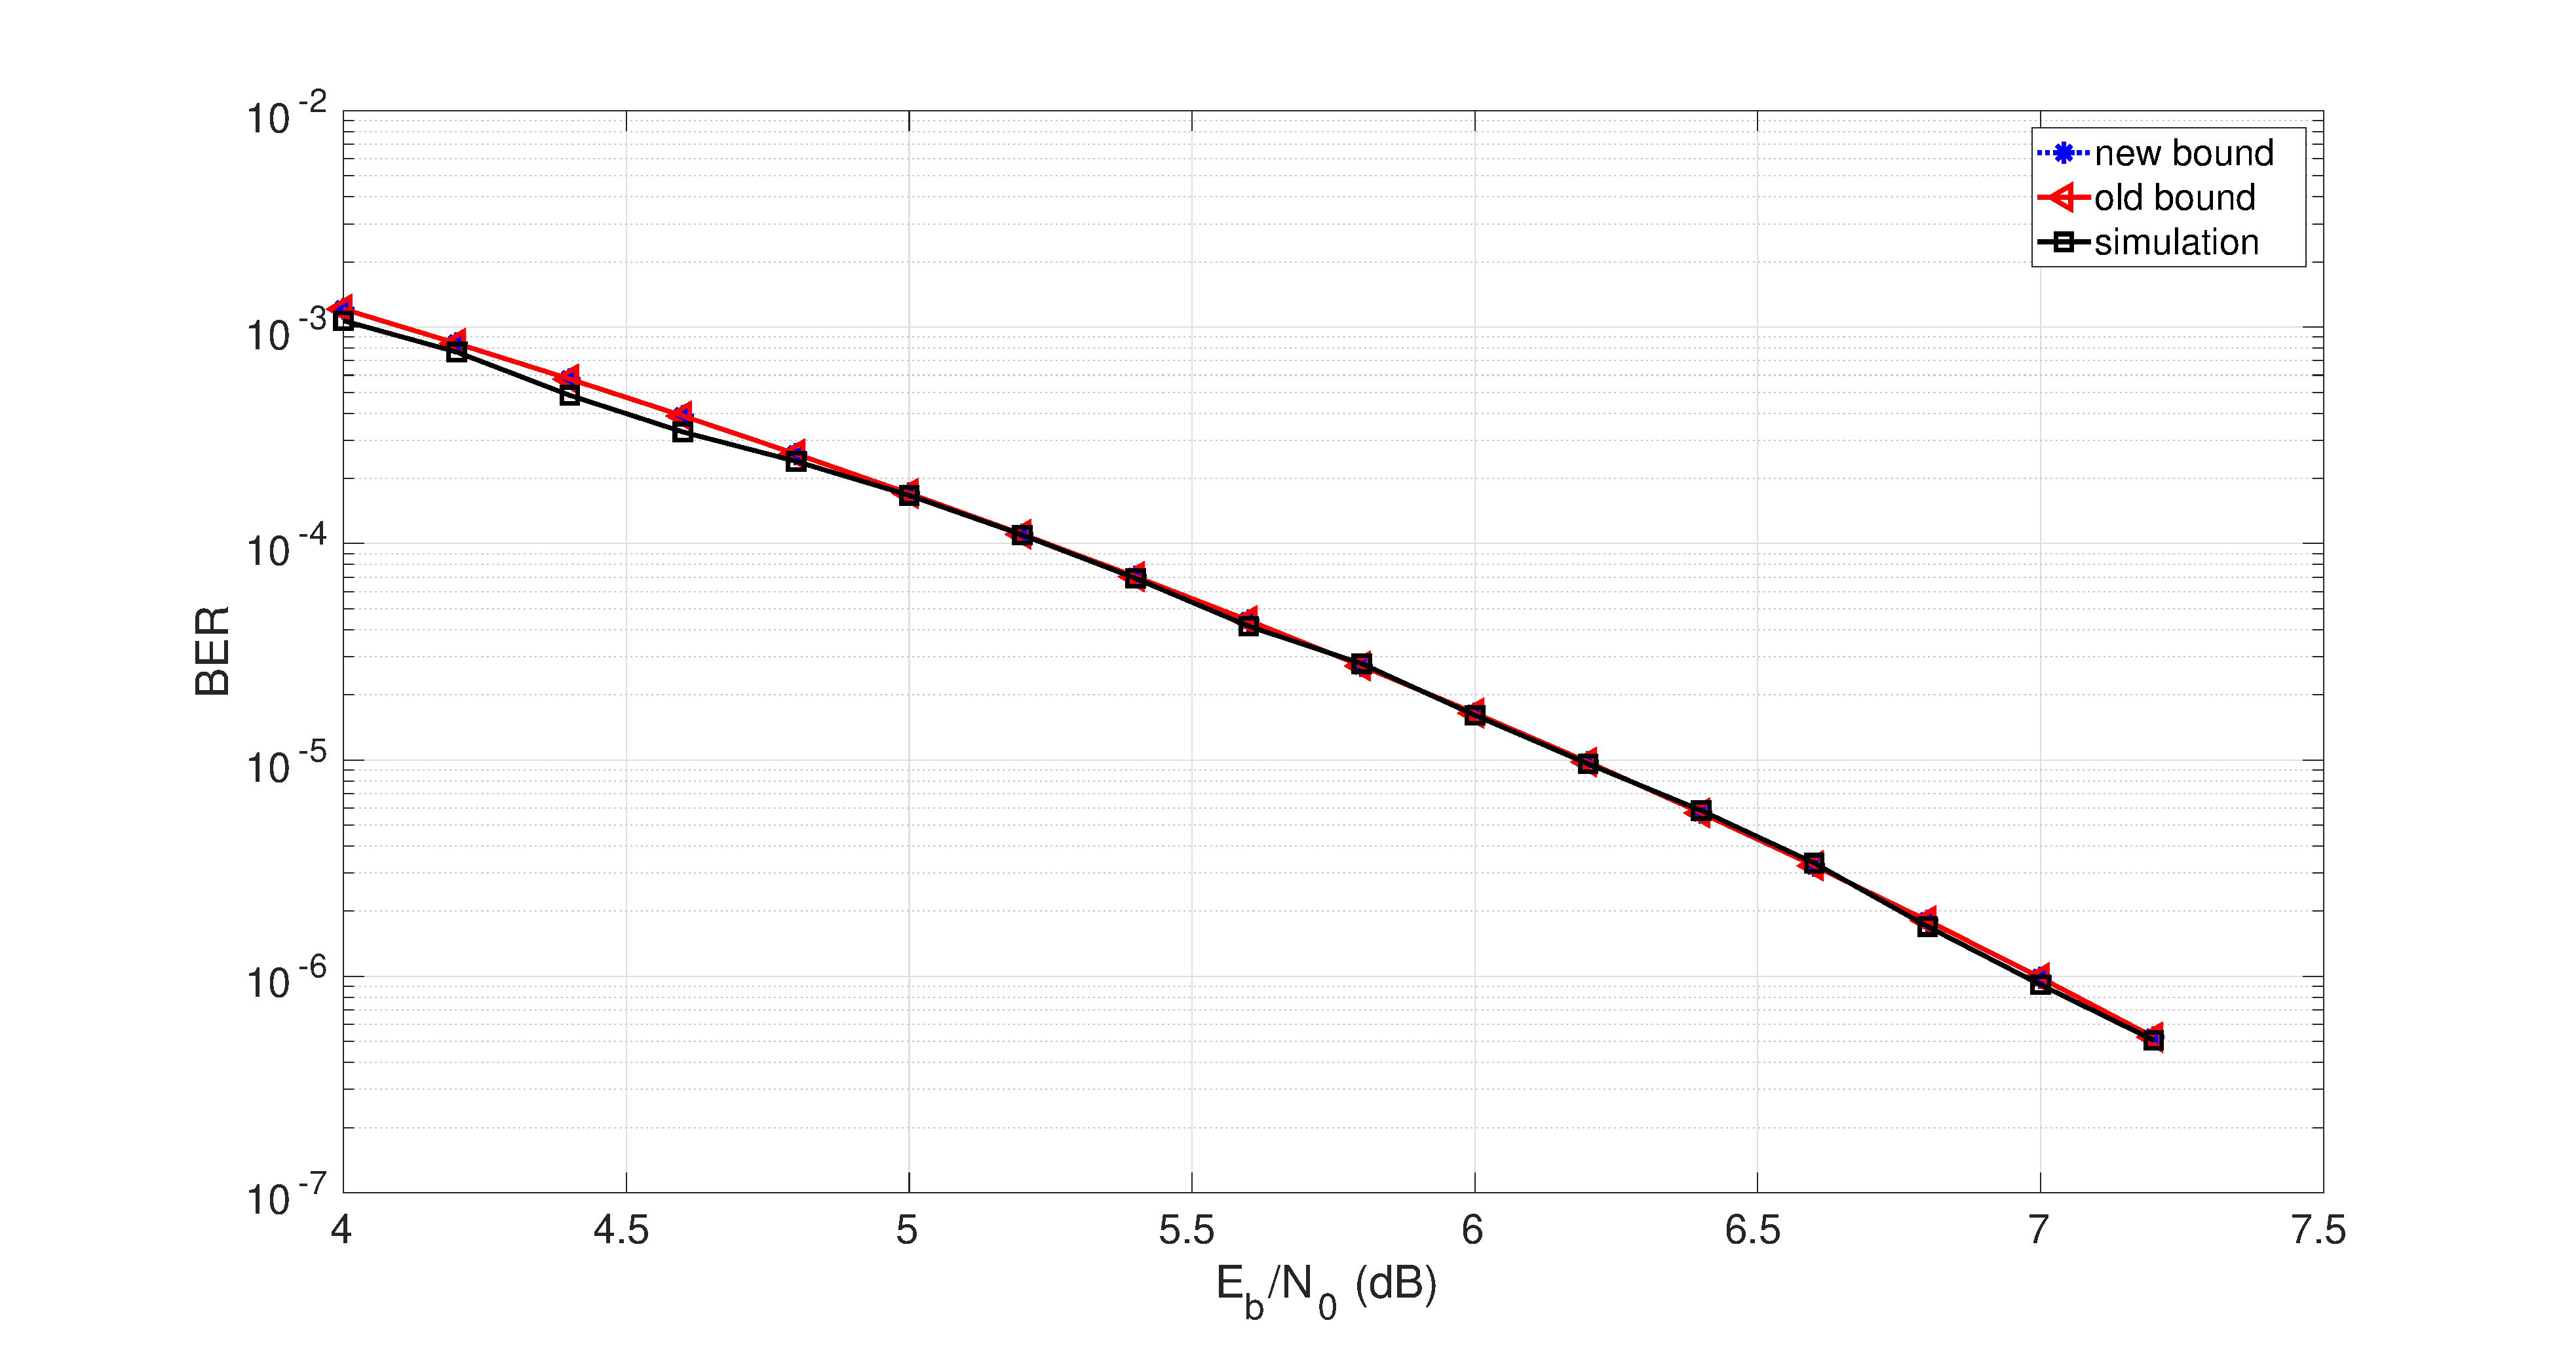
\includegraphics[width=0.8\textwidth]{./Images/RSC_5_7_higher_weights.eps}
%		\caption{Old Bound vs New Bound vs Simulation for 5/7 RSC Code, with higher weights }
%		\label{simFig4}
%		\end{figure}
		
		
%		\begin{figure}[h!]
%\centering
	%	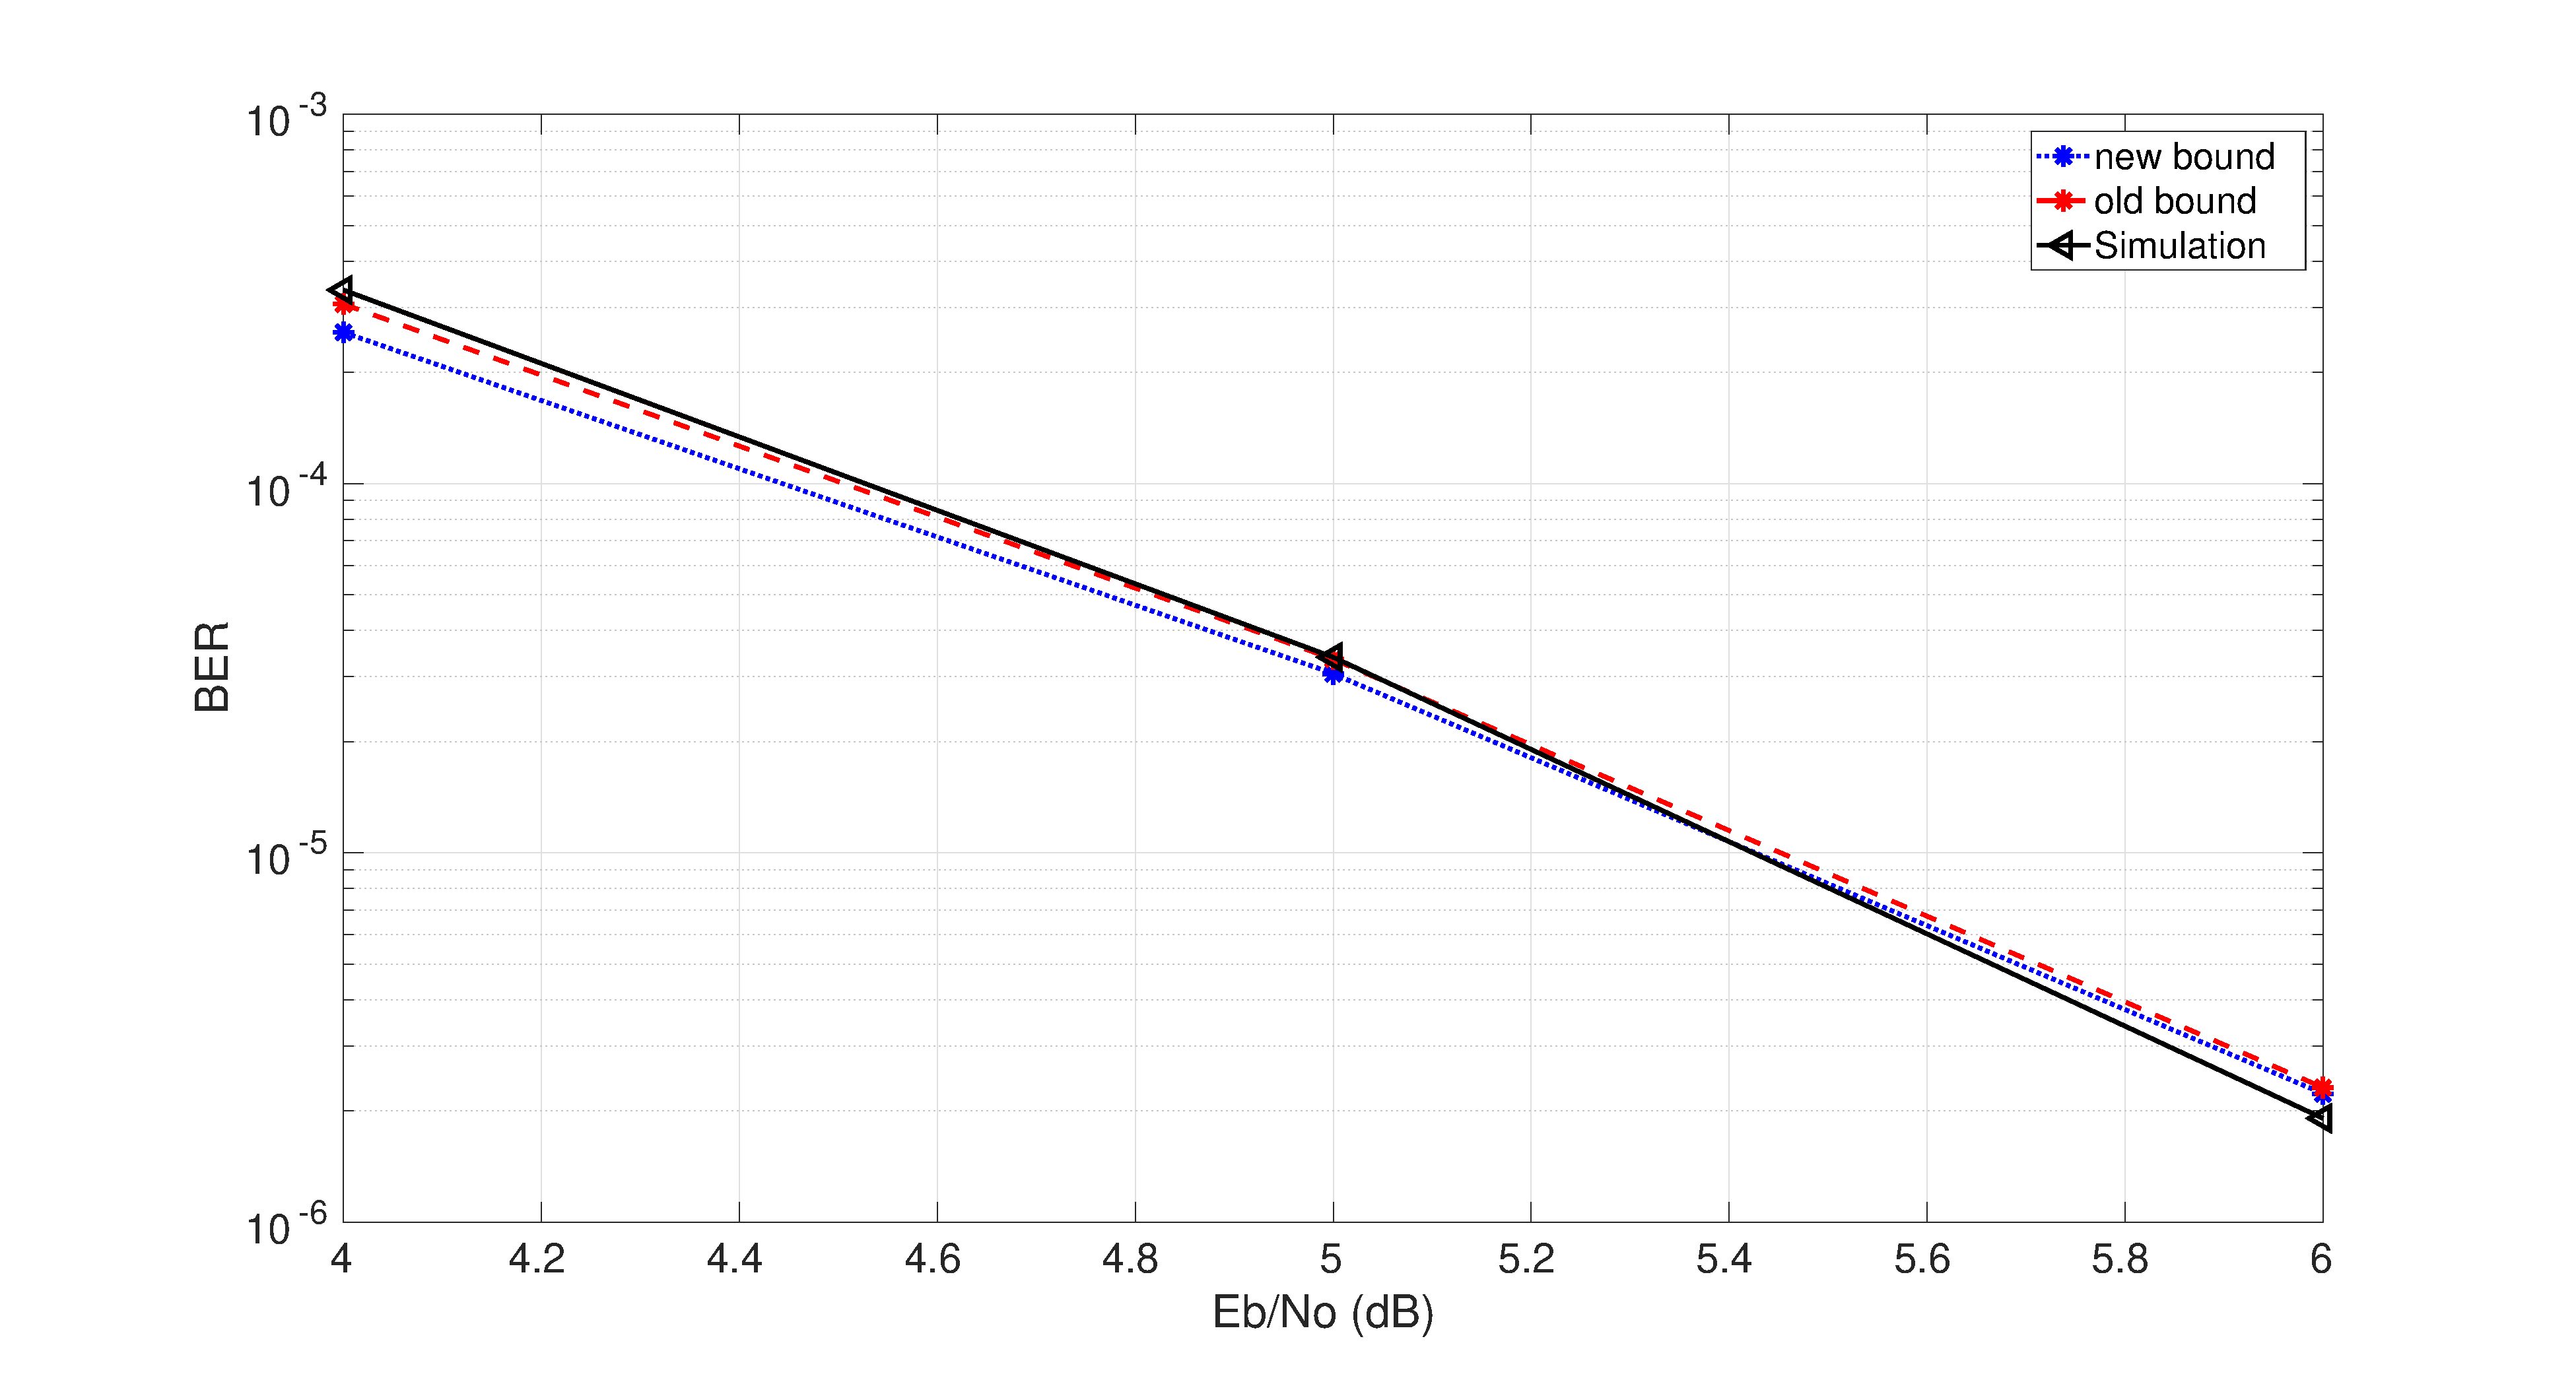
\includegraphics[width=0.5\textwidth]{./Images/RSC_37_21_v2.eps}
		%\caption{Old Bound vs New Bound vs Simulation for 37/21 RSC Code, with higher weights}
		%\label{simFig5}
		%\end{figure}



\newpage
\section{Conclusion}
\label{sec6}
In this paper, we proposed a novel method for  listing the patterns of the SCs and PCs ($2 \leq w_H(b(x)),w_H(h(x)) \leq 3$) of a low-weight RSC codeword, given the RSC code and a codeword cut-off weight, $d_{\text{max}}$.
Compared to the transfer function method, it has low complexity and the knowledge of the SC and PC patterns makes it a very useful for interleaver design. To validate our method, we compared the union bound obtained using our novel method with the union bound obtained via the transfer function as well as the simulation results for three RSC codes. Results suggest that RSC codes that can be sufficiently characterized by our novel method are much more attractive for use in TCs due to lower complexity required in the deterministic interleaver design.

%\newpage
\begin{thebibliography}{99}
\bibitem{ref1}  C. Berrou, A. Glavieux and P. Thitimajshima, "Near Shannon limit error-correcting coding and decoding: Turbo-codes. 1," Proceedings of ICC '93 - IEEE International Conference on Communications, Geneva, Switzerland, 1993, pp. 1064-1070 vol.2, doi: 10.1109/ICC.1993.397441.
\bibitem{ref2} John G. Proakis, Masoud Salehi. ``Digital Communications'', 
Fifth Edition,Chapter 8, McGraw-Hill.
\bibitem{ref3} Todd K. Moon. ``Error Correcting Codes'',Chapter 12, John Wiley \& Sons.
\bibitem{ref4}Alain Glavieux, ``Channel Coding in Communication Networks: From Theory to Turbocodes'',\\ Chapter 3, John Wiley \& Son. 
\bibitem{ref5} Jing Sun and O. Y. Takeshita, "Interleavers for turbo codes using permutation polynomials over integer rings," in IEEE Transactions on Information Theory, vol. 51, no. 1, pp. 101-119, Jan. 2005, doi: 10.1109/TIT.2004.839478.
%\bibitem{ref6} C. Berrou, Y. Saouter, C. Douillard, S. Kerouedan and M. Jezequel, "Designing good permutations for turbo codes: towards a single model," 2004 IEEE International Conference on Communications (IEEE Cat. No.04CH37577), Paris, France, 2004, pp. 341-345, doi: 10.1109/ICC.2004.1312507.
\bibitem{ref7}R. Garzón-Bohórquez, C. Abdel Nour and C. Douillard, "Protograph-Based Interleavers for Punctured Turbo Codes," in IEEE Transactions on Communications, vol. 66, no. 5, pp. 1833-1844, May 2018, doi: 10.1109/TCOMM.2017.2783971.
\bibitem{ref8}
S. Lu, W. Hou and J. Cheng, ”Input-output weight distribution of terminated RSC codes with limited codelength,” 2016
International Symposium on Information Theory and Its Applications (ISITA), Monterey, CA, USA, 2016, pp. 493-497.
\bibitem{ref9}
J. Deng, Y. Peng and H. Zhao, ”Distance spectrum calculation method for double binary turbo codes,” 2017 International
Conference on Recent Advances in Signal Processing, Telecommunications and Computing (SigTelCom), Da Nang, 2017,
pp. 98-102, doi: 10.1109/SIGTELCOM.2017.7849803.
\end{thebibliography}





\end{document}